\documentclass[10pt,a4paper]{article}
\usepackage[margin=2.2cm]{geometry}
\usepackage{lmodern}
\usepackage[T1]{fontenc}
\usepackage[utf8]{inputenc}
\usepackage{microtype}
\usepackage{graphicx}
\usepackage{booktabs}
\usepackage{tabularx}
\usepackage{longtable}
\usepackage{multirow}
\usepackage{makecell}
\usepackage{xcolor}
\usepackage{siunitx}
\usepackage{enumitem}
\usepackage{fancyhdr}
\usepackage{titlesec}
\usepackage{float}
\usepackage{caption}
\usepackage{lastpage}
\usepackage[most]{tcolorbox}
\usepackage{tikz}
\usetikzlibrary{arrows.meta,positioning,shapes.geometric,fit,calc,backgrounds}
\usepackage{listings}
\usepackage[hidelinks]{hyperref}

\definecolor{aigp}{HTML}{E8502F}
\definecolor{ink}{HTML}{1F2A44}
\definecolor{okgreen}{HTML}{2E7D32}
\definecolor{warnamber}{HTML}{B26A00}
\definecolor{badred}{HTML}{C62828}
\definecolor{soft}{HTML}{F4F6FA}

\sisetup{detect-all}
\setlist{itemsep=2pt,topsep=3pt}
\setlength{\parskip}{4pt}
\setlength{\parindent}{0pt}
\captionsetup{font=small,labelfont=bf}

\titleformat{\section}{\Large\bfseries\color{ink}}{\thesection}{0.6em}{}
\titleformat{\subsection}{\large\bfseries\color{ink}}{\thesubsection}{0.6em}{}
\titleformat{\subsubsection}{\normalsize\bfseries\color{ink}}{\thesubsubsection}{0.6em}{}

\pagestyle{fancy}
\fancyhf{}
\lhead{\small\color{gray}AI Grand Prix PQ --- Onboarding \& Engineering Journal}
\rhead{\small\color{gray}as of 16 Sep 2026}
\cfoot{\small\color{gray}\thepage}
\renewcommand{\headrulewidth}{0.3pt}

\lstset{basicstyle=\ttfamily\footnotesize,backgroundcolor=\color{soft},frame=single,rulecolor=\color{gray!40},breaklines=true,columns=fullflexible,keepspaces=true,showstringspaces=false}

\newtcolorbox{takeaway}[1][Key takeaways]{colback=aigp!6,colframe=aigp,fonttitle=\bfseries,title={#1},boxrule=0.6pt,arc=2pt,left=4pt,right=4pt,top=3pt,bottom=3pt}
\newtcolorbox{explain}[1][Plain-language explanation]{colback=soft,colframe=ink!60,fonttitle=\bfseries,title={#1},boxrule=0.4pt,arc=2pt,left=4pt,right=4pt,top=3pt,bottom=3pt}
\newtcolorbox{verdict}[1][Verdict]{colback=okgreen!5,colframe=okgreen!70!black,fonttitle=\bfseries,title={#1},boxrule=0.5pt,arc=2pt,left=4pt,right=4pt,top=3pt,bottom=3pt}
\newtcolorbox{warnbox}[1][Watch out]{colback=badred!4,colframe=badred!80!black,fonttitle=\bfseries,title={#1},boxrule=0.5pt,arc=2pt,left=4pt,right=4pt,top=3pt,bottom=3pt}

\newcommand{\V}{\textsuperscript{\textcolor{okgreen}{[V]}}}
\newcommand{\I}{\textsuperscript{\textcolor{warnamber}{[I]}}}
\newcommand{\X}{\textsuperscript{\textcolor{ink}{[ext]}}}
\newcommand{\code}[1]{\texttt{\detokenize{#1}}}

\begin{document}

%======================================================================== TITLE
\begin{titlepage}
\vspace*{1.5cm}
{\color{aigp}\rule{\linewidth}{2pt}}\\[0.6cm]
{\Huge\bfseries\color{ink} AI Grand Prix\\[0.25cm] Physical Qualifier}\\[0.4cm]
{\LARGE Onboarding Crash Course \& Engineering Journal}\\[0.4cm]
{\color{aigp}\rule{\linewidth}{2pt}}\\[0.8cm]
{\large Team Electric Fire (Team 10) \quad$\cdot$\quad repo \code{Code-Red-Cables/AI_GP}, branch \code{isaacsim} @ \code{66b61c5}}\\[0.3cm]
{\large Revision~1: 16 September 2026, the evening before the team arrived at LC3\\
\textbf{Revision~2: 17 September 2026, written on site with the real drone and the specification in hand}}\\[1.2cm]

\begin{tcolorbox}[colback=soft,colframe=ink!40,boxrule=0.4pt,arc=2pt,title=How to read this document,fonttitle=\bfseries]
\textbf{Part I (Sections 1--5)} is a crash course: what the competition is, the minimum drone-autonomy vocabulary, how our system is put together, where things live in the repo, and what the physical course looks like.
\textbf{Part II (Sections 6--12)} is the engineering journal: project history, the Isaac PPO stack in depth, audit findings with evidence, the durability (stress) study run on 16 Sep, Plan B, and next steps.

Evidence tags: \V\ verified by reading code, running it, or checking git on 16 Sep;
\I\ inference; \X\ from a public source outside our repo (organizer site, the Betaflight source, or the public repository of AI of Sauron, another PQ team).
The \code{AI_GP} repository was treated as \emph{read-only}; every experiment ran on scratch copies.

\textbf{People and plans named in this document.}
\begin{itemize}
\item \textbf{Gene} (Geneustace Wicaksono) is the team's main developer. He built and trained the simulator pilot described here.
\item \textbf{Plan~A:} fly Gene's trained neural network at racing speed.
\item \textbf{Plan~B:} fly a slower, hand-written step-by-step controller that stops and lines up in front of each gate (Section~\ref{sec:planbsim}).
\item \textbf{AI of Sauron:} another physical-qualifier team, from Georgia Tech, whose public repository describes the same drone.
\item \textbf{Where the files are:} every file this document mentions (the corrections patch, the test tools, the one-hour retrained model, the raw results) is in the \code{AI_GP} repository on the branch \code{pq-analysis-0916}, under \code{analysis/2026-09-16/}. The retrained model is at \code{isaac_drone_racer/models/pq_retrain_1h_corrected.pt}. All experiments ran on bojro's laptop (RTX 4060 laptop GPU, Windows with WSL).
\end{itemize}
\end{tcolorbox}

\vspace{0.6cm}
\begin{takeaway}[Summary]
\begin{enumerate}[leftmargin=1.2em]
\item \textbf{The course is fixed and known.} Ten numbered gates (gate~9 is a stacked double gate, gate~6 is a split-S), flown in order, two laps. Only small as-built differences from the published map are expected.
\item \textbf{What we had for the physical qualifier (PQ):} a neural-network pilot that Gene trained by reinforcement learning (trial and error in a simulator, explained in Section~\ref{sec:rl}). It is saved as the file \code{pq_speed_best.pt} and is called ``Gene's model'' throughout this document. In simulation it lapped in \textbf{7.35--7.47\,s}, averaging \SI{14.4}{m/s} and peaking at \SI{25.4}{m/s} (verified headless on 16 Sep). \textbf{As of 17 September this model is abandoned} --- it does not survive on the corrected simulator. It is kept in this document as evidence of \emph{how} a policy can look excellent and be worthless, which is the most useful thing it now does.
\item \textbf{Nothing in the repo talks to the real drone yet.} The team's flight program (the Python ``client'' in the repository root) speaks MAVLink, the protocol of the virtual-qualifier simulator; the real drone is Betaflight + MSP over UART to a Jetson. Camera capture, a real-image gate detector and an onboard gate counter are also still to be built.
\item \textbf{Four corrections for the team:}
  (a) a bug in the training code stops it from counting gate passes, so any further training fails (proven by a side-by-side test; the fix is one line);
  (b) the simulated camera is \SI{90}{\degree} wide, the real one is \SI{75}{\degree};
  (c) Gene's simulated course is about 93\,\% of the true size (it must be scaled up by about 7.5\,\%), and its gates sit \SI{0.65}{m} too high;
  (d) the real flight controller turns stick commands into rotation speed and thrust along curves, but the simulator assumes straight-line relationships.
\item \textbf{Durability:} the policy is fast but brittle.
\begin{itemize}
\item \textbf{Real camera:} 42 crashes per 100 gates.
\item \textbf{True course size:} 10 per 100.
\item \textbf{Both together:} it clears 4 gates and crashes, every time.
\item \textbf{After a one-hour retrain on the corrected simulator:} 10$\times$ fewer crashes under expected conditions, but still only 6--7\,\% two-lap success. A real retrain takes hours (Sections~\ref{sec:stress}--\ref{sec:retrain}).
\end{itemize}
\item \textbf{Strategy:} scoring is most gates first, time second, best run of Mon~21--Tue~22 Sep. Bank a valid run with Plan~B first, then attempt speed.
\item \textbf{Plan~B tested in simulation} (Section~\ref{sec:planbsim}), using the ``balanced'' setting: gates at \SI{2.5}{m/s}, cruise \SI{4}{m/s}. It finished \textbf{100\,\%} of runs under expected conditions and 88\,\% under rougher ones, in about \textbf{2:05} for two laps.
\begin{itemize}
\item ``Safe'' takes 2:21 (93\,\% under rougher conditions); ``fast'' takes 1:52 (79\,\% under rougher conditions).
\item A barometer is optional.
\item \textbf{Camera tilt must be measured:} an unknown \SI{5}{\degree} error is its biggest single risk.
\end{itemize}
\end{enumerate}
\end{takeaway}
\end{titlepage}

\tableofcontents
\newpage

%========================================================== STATUS 17 SEPTEMBER
\section*{Status at 17 September --- read this before anything else}
\addcontentsline{toc}{section}{Status at 17 September --- read this before anything else}

Revision~1 of this document was written on the evening of 16 September, off site, before anyone had
touched the drone. The team is now at LC3, the race drone has been weighed, and the physical-qualifier
specification (VADR-TS-005, issue 00.02) has been re-read line by line. Some of what follows in
Parts~I and~II has been overtaken. \textbf{Where this section disagrees with a later section, this
section is right.}

\subsection*{What changed}

\begin{table}[H]\centering\footnotesize
\begin{tabularx}{\linewidth}{@{}p{3.0cm}XX@{}}
\toprule
Item & Revision~1 said & Now \\
\midrule
Gene's model & The main line for Plan~A & \textbf{Abandoned.} It does not survive on the corrected simulator. Gene has reviewed the findings and agrees. The objective is now to train a new policy on the corrected simulator \\
Drone mass & \SI{0.6076}{kg} (the simulated value) & \textbf{\SI{1745}{g}} measured, race configuration. See the box below for why this matters less, and differently, than it looks \\
Camera & fx\,$\approx$\,424\,px (\SI{74.1}{\degree}), from another team's calibration & \textbf{fx\,=\,fy\,=\,417.0\,px} (\SI{75}{\degree}), from our own specification. Ours must still be calibrated --- the spec says no calibration matrices will be provided \\
Deployment layer & ``Also still to be built'' & Still the critical path, but \textbf{much smaller than feared}: the organizers ship a complete, working MSP layer on the drone (\code{~/target/msp/}), including a fake flight controller for offline development. Ours is the adapter, not the protocol \\
Link speed & Assumed our 60\,Hz policy rate was achievable & The organizers state twice that the link gives ``attitude at 30--50\,Hz; a hard real-time control loop is not'' realistic. \textbf{May force a retrain at a lower policy rate} \\
Camera mode & Assumed 1920$\times$1080 at 60\,fps & The carrier wires only \textbf{two of four} camera data lanes. That mode may not exist --- and the \SI{75}{\degree} figure is quoted \emph{for} it \\
``Next gate'' input & Not called out & \textbf{No source exists on the real drone.} The simulator supplied it \\
Safety pilot & Assumed possibly available during a run & \textbf{A valid run allows no human pilot intervention at all} (spec \S3.3). The override switch aborts a run; it cannot rescue one \\
Track footprint & $25.9\times\SI{50.25}{m}$ from the drawing's ruler & \textbf{Resolved.} The official gate-coordinate reference gives $85\times165$\,ft $=25.91\times\SI{50.29}{m}$, confirming the drawing. The spec's ``$60\times\SI{21}{m}$'' is wrong. Our corrected track matches the official table exactly \\
Compute machine & Gene's machine & \textbf{This laptop is now the primary simulation and test machine}, with cloud GPU rented for training \\
\bottomrule
\end{tabularx}
\end{table}

\subsection*{What is still true}

The durability study (Section~\ref{sec:stress}) stands, and its ranking is the most useful thing in
this document: \textbf{command delay and thrust calibration dominate every other error source}, with
camera field of view and camera tilt next. The gate-counting bug analysis (Section~\ref{sec:bug})
stands and the fix is applied. The map-audit method stands. Plan~B's logic and speed budget stand,
with the caveat that its numbers come from a purpose-built simulator, not from Isaac.

\begin{warnbox}[The weight finding, stated carefully --- this one is easy to get wrong]
The real drone is \SI{1745}{g}; the simulated one is \SI{607.6}{g}, an 8-inch airframe against a
5-inch one. The obvious response --- ``change the mass in the simulator and retrain'' --- is
\textbf{almost entirely wasted effort}, and doing it carelessly makes things worse.

The simulator converts a throttle command into a force by multiplying by the drone's own mass:
\code{thrust = (stick / hover\_stick) $\times$ mass $\times$ g}. Acceleration is force divided by
mass, so the mass cancels out. Change only the mass and the simulated drone flies identically.

Three things do \emph{not} cancel, and these are the real issues:
\begin{enumerate}
\item \textbf{Thrust-to-weight.} The simulator assumes the drone hovers at 25.5\,\% throttle, which
implies it can produce 3.5 times its own weight in thrust. That is a \SI{600}{g} racing quad's
figure. A \SI{1745}{g} machine carrying a Jetson more likely hovers near 35--45\,\%, i.e.\ about
2.0--2.6 times its weight. If so, the simulator has been promising the policy acceleration the drone
does not have. \textbf{Measuring this takes five minutes} (hover, read the throttle) and it is the
single most valuable number available today. For scale: a \SI{10}{\%} thrust error on its own took
crashes from about 2 to \textbf{58 per 100 gates} in the durability study.
\item \textbf{Rotational inertia.} The real airframe resists being rotated roughly \textbf{11--16
times} more than the simulated one (2.9$\times$ the mass, with arms about 2.2$\times$ longer, and
inertia grows with the square of the arm). \textbf{Danger:} the simulator's rate loop uses a fixed
gain \code{rate\_kp = 0.08}. If someone sets the real inertia and leaves that gain alone, the
simulated drone becomes about 13$\times$ more sluggish than anything real, and every policy trained
on it is worthless. That gain is not physics --- it stands in for Betaflight's own controller, which
is retuned for whatever airframe it is on. It must be re-derived from a measured response:
\code{gain $\approx$ inertia / measured response time}.
\item \textbf{Air drag}, which the simulator does not model at all.
\end{enumerate}
\end{warnbox}

\subsection*{The two gaps that block everything}

\begin{enumerate}
\item \textbf{Our flight client cannot talk to the real drone.} Searching the entire flight client
for ``MSP'' returns nothing; \code{controller.py} speaks MAVLink to the virtual qualifier's
simulator, which the real flight controller does not understand. \textbf{Much mitigated on 17
September:} the organizers ship a complete MSP layer on the board (\S\ref{sec:provided}), so what
remains is an adapter, the Betaflight curve inversion and the sign/axis mapping --- hours rather than
days, and testable on a laptop against their fake flight controller. Still the critical path.

\item \textbf{Nothing tells the drone which gate is next.} The policy's input includes a list of 18
on/off flags meaning ``this is the gate you are going for''. In the simulator that came free, from
the simulator. On the real course we must count gates ourselves from the camera --- and the double
gate counts twice per lap, which is exactly where a counter loses its place.
\end{enumerate}

\begin{warnbox}[New on 17 September: the link may be slower than our policy]
The organizers' software guide states, twice and emphatically, that the flight-controller link is
\emph{telemetry-grade}: ``MSP is request/response over a 115200-baud serial line. You poll; the FC
answers. Attitude at 30--50\,Hz is realistic; a hard real-time control loop is not.''

Our policy runs at \textbf{60\,Hz} and takes gyro readings as part of its input. Sending stick
commands at 60\,Hz is fine --- that is exactly what a radio link does, and Betaflight keeps the fast
stabilisation loop internally, which is where it belongs. The problem is the \emph{feedback} half: if
gyro only arrives at 30--50\,Hz, the simulator has been training the policy against a sensor faster
than the one it will fly with.

\textbf{Action:} measure the achievable rate on day one with the organizers' own
\code{companion\_listener\_msp.py}, then set the simulator's decimation to match \emph{before}
committing to a long training run. At 120\,Hz physics, decimation 2 gives 60\,Hz, 3 gives 40\,Hz and
4 gives 30\,Hz.
\end{warnbox}

\subsection*{What the organizers already provide}\label{sec:provided}

Everything below is pre-installed in \code{~/target/} on the Jetson. No pip, no network, no root.
Log in over a USB cable: \code{ssh dcl@192.168.55.1}, password \code{dcl}.

\begin{itemize}\sloppy
\item \code{msp/msp.py} --- \code{MSPLink}: all MSP framing, plus \code{attitude()},
\code{raw\_imu()}, \code{analog()}, \code{rc\_channels()}, \code{motors()}, \code{status()} and
arming-blocker decoding. Thread-safe, background receive loop, counts corrupt frames rather than
crashing on them.
\item \code{msp/msp\_rc.py} --- \code{RCTransmitter}: streams stick commands at a fixed rate from a
background thread \textbf{with a watchdog already built in}. Stop calling \code{set\_control()} and
it falls back to an idle frame by itself. \code{arm()} refuses unless throttle is at minimum;
\code{close()} disarms cleanly.
\item \code{msp/fake\_fc.py} --- \textbf{simulates a Betaflight flight controller on a laptop}, with
deliberate fault modes (frozen, saturated, wrong scale, no accelerometer, bus errors). The whole test
suite runs with nothing plugged in.
\item \code{msp/setup\_jetson\_uart.sh} --- frees the serial port from Linux's login console.
\textbf{Run once per board before anything else}; skipping it looks exactly like a dead flight
controller.
\item \code{msp\_bench.py} (info / telemetry / rc / demo), \code{imu\_check.py} (a real functional
IMU test, not just ``did it reply''), \code{companion\_listener\_msp.py} (live telemetry, and it
reports the achievable poll rate).
\item Camera: \code{live-view.py}, \code{live-view-pts.py} (hardware capture timestamps),
\code{live-view-imu.py}, \code{show-camera.py}, \code{raw-view.py}, \code{frame-timestamps.py}, plus
\code{bringup-check.sh} and \code{camera-bind-check.sh}.
\end{itemize}

The guide says it plainly: \textbf{``do not re-implement MSP framing.''}

\textbf{First action for whoever reaches a board:} \code{scp -r dcl@192.168.55.1:~/target ./}, and
share it --- that is what lets the rest of the team write and test adapter code without the drone.

\begin{warnbox}[Three constraints from those guides that will otherwise cost an afternoon each]
\begin{enumerate}
\item \textbf{Only two of the camera's four data lanes are wired} on this carrier, capping resolution
$\times$ framerate. Run \code{v4l2-ctl -d /dev/video0 -{}-list-formats-ext} and believe that list, not
the datasheet. The \SI{75}{\degree} field of view is quoted for 1920$\times$1080 at 60\,fps.
\item \textbf{The image processor needs a graphics context.} Colour, auto-exposure and white balance
run in NVIDIA's ISP, which fails over a plain SSH session and falls back to a flat, dim software
debayer. That is documented behaviour, not a broken camera.
\item \textbf{No deep-learning framework is installed.} OpenCV (GStreamer-enabled), NumPy, pyserial
and python3-gi --- no PyTorch. This makes the NumPy policy runtime \emph{mandatory}. And never
\code{pip install opencv-python}: it silently replaces the GStreamer build and the camera pipeline
then fails with no error text.
\end{enumerate}
There is also \textbf{no hardware sync wire between the camera and the flight controller}. Their
guide calls its camera--IMU timing section ``the section most likely to save you a week''. It is
right; read it before building anything that fuses the two.
\end{warnbox}

\subsection*{Where the working documents are}

This PDF is the onboarding and history document. The live operational plan is kept as Markdown in
the workspace root, because it changes daily:
\code{FIELD\_PLAN.md} (workstreams, procedures, schedule, contingencies),
\code{SIM\_MEASUREMENTS.md} (every parameter the simulator guesses and how to measure it),
\code{INSTALL\_PLAN.md} (what to install and download, ordered by how badly it blocks us),
\code{PLAN\_B.md} (the slow fallback).
Sections~\ref{sec:gaps}--\ref{sec:schedule} of this document summarise them.

\newpage

%======================================================================== PART I
\part*{Part I --- Crash course}
\addcontentsline{toc}{part}{Part I --- Crash course}

\section{The competition in two pages}

\subsection{What the AI Grand Prix is}
An autonomous drone-racing competition run by Anduril with the Drone Champions League (DCL); the drones come from Neros.\X\ More than 3{,}000 teams entered. Human input during a timed run disqualifies it: the drone must fly itself.

\begin{table}[H]\centering\small
\begin{tabularx}{\linewidth}{@{}lp{3.1cm}X@{}}
\toprule
Stage & When & What \\
\midrule
VQ1 (virtual qualifier 1) & opened 31 May & DCL ``FlightSim'' simulator on Windows; short course; spec VADR-TS-001. \\
VQ2 & 29 Jun -- 3 Aug & Harder course, position and attitude data blocked: camera (640$\times$360) + IMU only. Top 10 teams advanced.\X \\
\textbf{Physical Qualifier (PQ)} & \textbf{15--22 Sep 2026} & Real drones in a hall at Anduril LC3 (OC-23, 3100 W Lake Center Dr, Santa Ana). Spec VADR-TS-005 (issue 00.02). \\
Finals (``AI Grand Prix Ohio'') & November 2026 & Columbus, Ohio; live head-to-head; \$500K prize pool; top 10 at Ohio get at least \$5K.\X\ How many PQ teams advance is not published. \\
\bottomrule
\end{tabularx}
\caption{Competition stages.}
\end{table}

\subsection{PQ rules that matter}
\begin{itemize}
\item \textbf{Scoring} (spec \S3.3): rank by the \emph{maximum number of successfully passed gates}; tie-break is the \emph{fastest elapsed time to the last validly crossed gate}. Qualification uses the best result from the \textbf{final two days} (Mon~21 and Tue~22 Sep).
\item \textbf{A run} is two laps. Timing starts at the first timing line or gate trigger. Any pilot intervention makes the run invalid.
\item \textbf{Practice:} several dedicated slots per team per day (15\,min each in the earlier public spec TS-004\X) plus time in a training cage. Manual piloting is allowed in practice.
\item \textbf{Fleet:} each team gets 4 drones. Neros repairs them and does all charging; personal chargers are not allowed.
\item \textbf{Flight controller access:} rates, PIDs, filters and telemetry may be changed through the Betaflight CLI; reflashing is not allowed.
\item \textbf{Safety:} a pilot's RC transmitter always overrides autonomy. Nobody stands near the flight path. The safety briefing on day~1 is mandatory.
\item \textbf{Logistics:} 07:00--22:00 on site, out by 23:00, day badges, closed-toe shoes. Team 10 has its own password on the ``AI Grand Prix'' racing Wi-Fi. That password is in the welcome packet and must never go into the public repo.
\end{itemize}

\subsection{The hardware you will fly}
\begin{table}[H]\centering\small
\begin{tabularx}{\linewidth}{@{}lX@{}}
\toprule
Airframe & Neros Archer B2, 8-inch propellers (4.1 pitch). \textbf{All-up race weight measured on site, 17 Sep: \SI{1745}{g}.}\V\ Motor and battery specs are given on site. \\
Flight controller & Betaflight. Another PQ team reads firmware 4.4.3 on an H743 board, MSP API 1.45.\X \\
FC $\leftrightarrow$ computer & UART using \textbf{MSP} (MultiWii Serial Protocol), not MAVLink. Another team uses \code{/dev/ttyTHS1} at 115200 baud and sees about 100 MSP replies/s in total.\X \\
Computer & NVIDIA Jetson Orin NX 16\,GB on a Seeed A603 carrier, JetPack 6.2 (Ubuntu 22.04, Python 3.10), 25\,W mode, full root access. The organizers provide demo apps for camera bring-up and FC serial communication. \\
Camera & Arducam 12.3\,MP HQ (Sony IMX477), rolling shutter, M12 lens, 1920$\times$1080. Spec: 60\,fps and \SI{75}{\degree} horizontal FOV, which is \textbf{fx\,=\,fy\,=\,417.0\,px} at 640$\times$360. Another team calibrated \emph{their} lens at fx\,$\approx$\,1271\,px (\SI{74.1}{\degree}), which is close but is their lens, not ours. Tilt is adjustable \emph{in flight}, exposure and gain are controllable, and \textbf{no calibration matrices are provided} --- so we must calibrate our own. \\
IMU & From Betaflight, calibrated at power-on. Spec says 50\,Hz; about 92\,Hz is achievable over MSP.\X \\
Positioning & None: no motion capture, no GPS. \\
\bottomrule
\end{tabularx}
\caption{PQ hardware (spec VADR-TS-005 \S3.6--3.8 and FAQ).}
\end{table}

\subsection{Is the course the same as in our simulator? (FAQ)}
\begin{explain}[Short answer: yes, it is a fixed, published course]
The organizers publish one layout: the plan on page~6 of our spec, plus a gate-coordinate table (``Drone Racing Track --- Gate Layout \& Coordinate Reference for Contestants'').
The course is built once in the hall and is the same for every team; it is \emph{not} randomized between runs. Our Isaac track is a hand-digitized copy of that plan, slightly mis-scaled (Section~\ref{sec:track}).

What can differ in practice:
(i) as-built placement a few tens of centimetres or a few degrees off the drawing;
(ii) gates knocked and re-set during the week;
(iii) exact heights, which the plan does not give (frames stand on the floor, so the opening centre is about \SI{1.35}{m}; the double gate's upper opening is about \SI{4.05}{m}, confirmed on site on 15 Sep by another team\X);
(iv) the spec says map-distribution details ``will be announced later'', so ask whether the layout can change before scoring.
This is why the durability study treats ``gate shifted a little'' as \emph{expected}, while ``a different course'' is only a stress probe.
\end{explain}

%------------------------------------------------------------------------
\section{Drone-racing autonomy in ten minutes}

\subsection{The loop}
Every autonomous racer runs the same loop many times per second:
\begin{enumerate}
\item \textbf{Perceive.} Find the gates in the camera image. Our stack describes a gate by its \textbf{8 keypoints}: the 4 corners of the 2.7\,m outer frame and the 4 corners of the 1.5\,m opening.
\item \textbf{Estimate.} Know your own attitude (roll, pitch), rotation rates (gyro) and, roughly, your velocity. There is no position sensor, so the gate itself is the landmark.
\item \textbf{Decide.} A controller or learned \textbf{policy} maps what it sees to a command.
\item \textbf{Actuate.} Send the command to the flight controller (FC), which spins the motors.
\end{enumerate}

\subsection{Vocabulary}
\begin{longtable}{@{}p{3.3cm}p{12.3cm}@{}}
\toprule
Term & Meaning \\
\midrule\endhead
Roll / pitch / yaw & Rotation about the forward / right / down axes. Roll and pitch tilt the thrust to move sideways and forward; yaw turns the nose. \\
Body rates & How fast the drone rotates (rad/s) about each axis. The gyro measures them. \\
ACRO mode & Betaflight mode in which the sticks command \emph{body rates}. Fastest and most agile. Our policy is trained for this. \\
ANGLE mode & Betaflight mode in which the sticks command \emph{tilt angles} and the FC self-levels. Safer and slower. Plan~B uses it. \\
Throttle / collective & Total thrust. ``Hover stick'' is the throttle value that exactly holds altitude. \\
MSP & MultiWii Serial Protocol. Betaflight's command/telemetry protocol over a serial link. \\
MSP override & Betaflight feature: while an AUX switch is on, selected RC channels come from the companion computer over MSP instead of the pilot's radio. \\
MAVLink & A different drone protocol (PX4/ArduPilot). The VQ simulator used it, which is why our client speaks it. \\
Jetson & The onboard NVIDIA computer that runs our code. \\
Keypoints & The 8 gate corners in pixel coordinates. \\
PnP & Perspective-n-Point: solve the camera's pose relative to an object from its known 3-D corners and their pixel positions. \\
FOV / fx & Field of view, and focal length in pixels. Narrower FOV means larger fx and larger-looking gates. \\
Latency & Delay from photon hitting the sensor to motor response. \\
RL / PPO & Reinforcement learning: the policy learns by trial and error from a reward. PPO (Proximal Policy Optimization) is the algorithm we use. \\
Policy / checkpoint & The trained neural network, and the file that stores its weights (\code{.pt}). \\
Observation / action & What the policy sees / what it outputs. \\
Reward shaping & Extra reward terms that guide learning (e.g.\ ``progress toward the gate''). \\
Privileged information & Information a simulator has that the real drone does not, e.g.\ exact gate corners. \\
Sim-to-real gap & Everything that differs between simulation and reality. \\
Domain randomization & Varying the simulator during training (mass, delays, noise) so the policy tolerates reality. \\
Isaac Sim / Isaac Lab & NVIDIA's GPU physics simulator, and its robot-learning framework (thousands of drones in parallel). \\
skrl & The RL library used to run PPO. \\
Keeper & The team's word for the saved model currently worth keeping; here, Gene's model \code{pq_speed_best.pt}. \\
Episode / attempt & One simulated flight, from its start until a crash or the time limit. \\
Plant & The simulator's model of how the drone physically responds to commands. \\
Headless & Running the simulator without its 3-D window. \\
Fine-tune / warm start & Continue training from an existing saved model instead of from scratch. \\
IMU & Inertial measurement unit: the gyroscope (rotation speed) and accelerometer on the flight controller. \\
Betaflight & The flight-controller firmware on the drone. It stabilizes the drone and turns stick commands into motor speeds. \\
UART / serial & The cable link between the Jetson computer and the flight controller. \\
AUX channel & An extra radio channel driven by a switch on the pilot's transmitter (for example ARM on AUX1). \\
Bitmask & A number whose binary digits switch individual options on or off (the override mask 15 = binary 1111 = roll, pitch, throttle and yaw). \\
Failsafe & What the flight controller does when it loses its command link; here \code{DROP} cuts the motors. \\
PID & A standard feedback controller that corrects an error using its size, its accumulated history and its rate of change. \\
Barometer & An air-pressure sensor that gives altitude. \\
Dead reckoning & Estimating position by integrating motion estimates, with no external reference; errors grow over time. \\
Gate normal / axis & The direction a drone must fly through a gate, perpendicular to the gate frame. \\
p95 & The 95th percentile: 95\,\% of values are at or below it. \\
Intrinsics / calibration & A camera's focal length, image centre and lens distortion, measured with a printed pattern (for example a ChArUco board). \\
YOLO / HSV detector & Two ways to find gates in an image: a neural-network detector (YOLO) or a colour threshold (HSV). \\
TensorRT / GStreamer & NVIDIA's tool for running neural networks fast on the Jetson; a video pipeline library for reading the camera. \\
\bottomrule
\end{longtable}

%------------------------------------------------------------------------
\section{How our system works}\label{sec:system}

\subsection{Big picture}
\begin{figure}[H]\centering
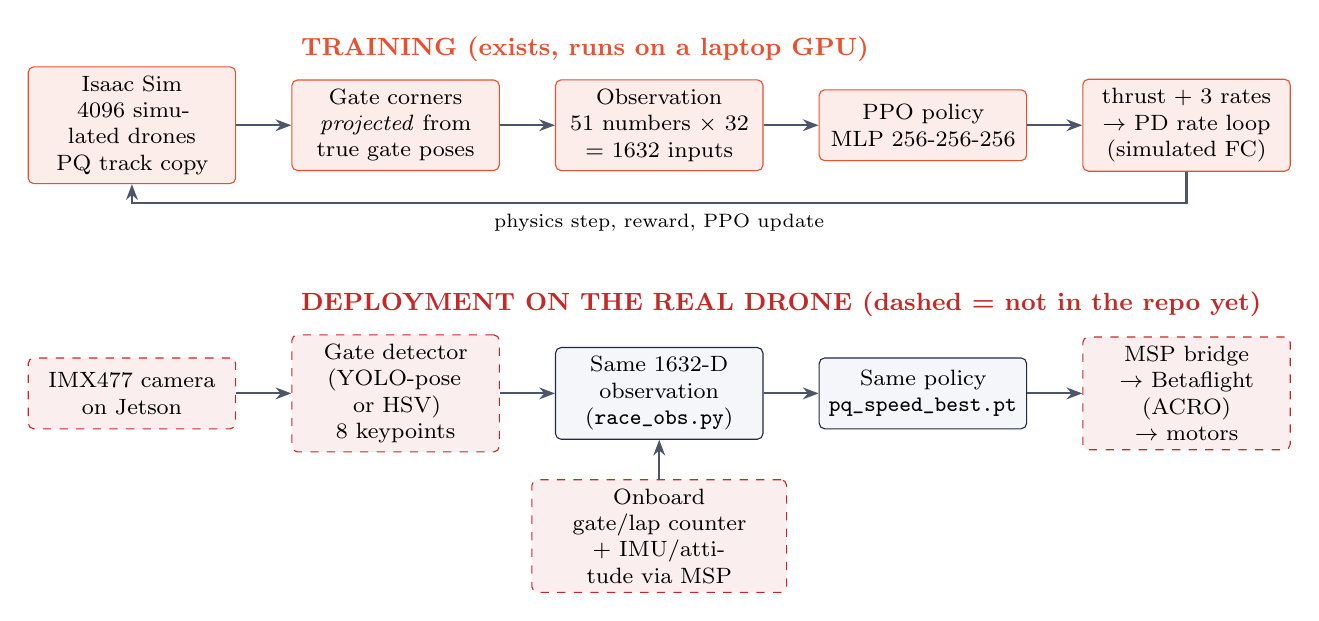
\begin{tikzpicture}[
  node distance=5mm and 7mm,
  box/.style={draw=ink,rounded corners=2pt,fill=soft,align=center,font=\footnotesize,minimum height=9mm,text width=24mm},
  sim/.style={box,fill=aigp!10,draw=aigp},
  todo/.style={box,fill=badred!8,draw=badred,dashed},
  arr/.style={-{Stealth[length=2mm]},thick,draw=ink!80}]
% training row
\node[sim] (isaac) {Isaac Sim\\4096 simulated drones\\PQ track copy};
\node[sim,right=of isaac] (proj) {Gate corners\\\emph{projected} from\\true gate poses};
\node[sim,right=of proj] (obs) {Observation\\51 numbers $\times$ 32\\= 1632 inputs};
\node[sim,right=of obs] (pol) {PPO policy\\MLP 256-256-256};
\node[sim,right=of pol] (act) {thrust + 3 rates\\$\rightarrow$ PD rate loop\\(simulated FC)};
\draw[arr] (isaac)--(proj); \draw[arr] (proj)--(obs); \draw[arr] (obs)--(pol); \draw[arr] (pol)--(act);
\draw[arr] (act.south) -- ++(0,-4mm) -| node[pos=0.25,below,font=\scriptsize]{physics step, reward, PPO update} (isaac.south);
\node[above=1mm of proj.north west,anchor=south west,font=\small\bfseries,color=aigp] {TRAINING (exists, runs on a laptop GPU)};
% deployment row
\node[todo,below=22mm of isaac] (cam) {IMX477 camera\\on Jetson};
\node[todo,right=of cam] (det) {Gate detector\\(YOLO-pose or HSV)\\8 keypoints};
\node[box,right=of det] (obs2) {Same 1632-D\\observation\\(\code{race_obs.py})};
\node[box,right=of obs2] (pol2) {Same policy\\\code{pq_speed_best.pt}};
\node[todo,right=of pol2] (msp) {MSP bridge\\$\rightarrow$ Betaflight (ACRO)\\$\rightarrow$ motors};
\draw[arr] (cam)--(det); \draw[arr] (det)--(obs2); \draw[arr] (obs2)--(pol2); \draw[arr] (pol2)--(msp);
\node[todo,below=5mm of obs2,text width=30mm] (cnt) {Onboard gate/lap counter\\+ IMU/attitude via MSP};
\draw[arr] (cnt)--(obs2);
\node[above=1mm of det.north west,anchor=south west,font=\small\bfseries,color=badred] {DEPLOYMENT ON THE REAL DRONE (dashed = not in the repo yet)};
\end{tikzpicture}
\caption{Training vs deployment. The policy and observation format are shared; the dashed blocks are the missing deployment layer.}
\end{figure}

\subsection{Reinforcement learning in plain terms}\label{sec:rl}
\begin{explain}[How Gene's model was made]
\begin{itemize}
\item \textbf{The pilot is a neural network}, called the \emph{policy}. Many times per second it receives a list of numbers describing what the drone currently senses (the \emph{observation}) and outputs four numbers: throttle and three rotation speeds (the \emph{action}).
\item \textbf{Nobody tells it how to fly.} It starts out flying randomly inside a simulator. After every step the simulator hands out a score, the \emph{reward}: points for moving toward the next gate and for passing through it, and a penalty for crashing.
\item \textbf{The training algorithm, PPO} (Proximal Policy Optimization), slowly adjusts the network's internal numbers so that actions which earned more reward become more likely.
\item \textbf{Scale:} Isaac Sim runs thousands of simulated drones in parallel on the graphics card (4096 in Gene's runs).
\begin{itemize}
\item A \emph{timestep} is one decision made by all of those drones at once.
\item \emph{Samples} are timesteps multiplied by the number of drones.
\item One of Gene's typical training runs is 50{,}000 timesteps, about 205 million samples, about 1.4 hours.
\end{itemize}
\item \textbf{Checkpoints:} the saved network is a \emph{checkpoint} file (\code{.pt}). Training runs can start from an earlier checkpoint instead of from scratch (a \emph{warm start} or \emph{fine-tune}).
\item \textbf{The key limitation:} the network only learns to handle what the simulator showed it. If the simulator's course, camera, delays or thrust differ from reality and were never varied during training, the network has no reason to cope with the difference. Section~\ref{sec:stress} measures exactly this.
\end{itemize}
\end{explain}

\subsection{What the policy sees and does}\label{sec:obs}
\begin{table}[H]\centering\small
\begin{tabularx}{\linewidth}{@{}lXX@{}}
\toprule
Slots & Content & Notes \\
\midrule
0--15 & where the 8 gate corners appear in the camera image (horizontal and vertical pixel position, divided by the image size 640$\times$360) & $-1$ if a corner is not visible; order: outer frame top-left, top-right, bottom-right, bottom-left, then the same for the inner opening \\
16--23 & visibility flags & corner in front of camera and within frame $\pm$15\,\% \\
24--25 & roll, pitch (rad) & gravity-referenced \\
26--28 & rotation speeds from the gyroscope, limited to $\pm$8 rad/s & \\
29--31 & ``commanded'' body velocity & integrated from thrust, attitude and a drag model; never from the accelerometer \\
32--49 & which gate is next: 18 numbers, all 0 except a single 1 at that gate's position (11 of the 18 slots are used on this course) & the policy always knows which gate it is flying to \\
50 & progress through the course: gate number divided by 17 (the list has 18 slots, numbered 0--17) & \\
\bottomrule
\end{tabularx}
\caption{One observation frame (51 numbers). The policy receives the last 32 frames (0.53\,s at 60\,Hz): 1632 inputs. Keypoints refresh at 30\,Hz; everything else at 60\,Hz.}
\end{table}

\begin{explain}[How the model is structured]
\begin{itemize}
\item \textbf{Network:} a plain feed-forward net, $1632 \rightarrow 256 \rightarrow 256 \rightarrow 256$ (ELU), with a 4-number action head and a 1-number value head (551k parameters). Inputs are normalised by stored running means and variances.
\item \textbf{Output:} $[-1,1]^4$, decoded to
  \begin{itemize}
  \item a throttle stick: hover at 0.255, range 0.05--0.90, mapped linearly to newtons with a \SI{0.6076}{kg} mass (maximum thrust-to-weight $\approx3.5$);
  \item three body rates of up to $\pm$\SI{3.2}{rad/s}.
  \end{itemize}
\item \textbf{No map input,} but the ``which gate is next'' numbers tell it \emph{where on the course} it is. That is how it learns this specific course's turns. It also means a different course, or a wrong gate count on the real drone, will confuse it.
\end{itemize}
\end{explain}

\subsection{How it was trained}
\begin{itemize}
\item \textbf{Timing:} 120\,Hz physics, 60\,Hz policy, 40\,s episodes, a random start gate each episode, tiny random pushes ($\pm$0.1\,N).
\item \textbf{Plant:} rigid body with collective thrust plus a PD body-rate loop ($k_p{=}0.08$, $k_d{=}0.003$, moment limits 0.30/0.30/0.20\,N$\cdot$m). No motor model, no drag, no latency, no sensor noise.
\item \textbf{Episode ends on:} collision (including the ground), crossing a gate plane outside the $\pm$0.75\,m opening, more than 20\,m from the target gate, or the 40\,s time-out.
\item \textbf{PPO settings (technical; safe to skip):} 4096 envs, 24-step rollouts, learning rate $10^{-4}$ (KL-adaptive), $\gamma{=}0.99$, $\lambda{=}0.95$, 50k timesteps per run ($\approx$1.4\,h on Gene's RTX 4070 laptop with 4096 drones).
\end{itemize}

\begin{table}[H]\centering\small
\begin{tabularx}{\linewidth}{@{}XrX@{}}
\toprule
Reward term & Weight & Idea \\
\midrule
gate passed & +600 & the real objective \\
progress toward the next gate / toward a point 3\,m straight in front of it & +20 / +25 & continuous guidance toward the gate \\
speed along the gate normal at the crossing & +3.4 & go fast through gates \\
camera aligned / centred at crossing & +4 / +4 & pass cleanly \\
low-gate dive, proximity, heading, look-at, visible & small & shaping \\
time penalty, angular-rate penalty & $-0.01$, $-10^{-4}$ & \\
termination (crash, miss, flyaway) & $-100$ & \\
\bottomrule
\end{tabularx}
\caption{Reward terms: the points the simulator awards during training (current code, identical to the settings Gene's model was trained with).}
\end{table}

%------------------------------------------------------------------------
\section{Repo tour}\label{sec:repo}
\begin{table}[H]\centering\footnotesize
\begin{tabularx}{\linewidth}{@{}p{6.6cm}X@{}}
\toprule
Path (branch \code{isaacsim}) & What it is \\
\midrule
\code{ISAACSIM.md} & Start here for the PQ stack: Windows GUI play, WSL headless training, installs \\
\code{isaac_drone_racer/} & The Isaac Lab project (fork of kousheekc/isaac\_drone\_racer, copied in without its git history) \\
\quad \code{tasks/drone_racer/drone_racer_env_cfg.py} & Scene, \textbf{track}, observation, rewards, terminations, task settings \\
\quad \code{tasks/drone_racer/mdp/} & Actions (plant), commands (gate targeting, pass detection), observations, rewards, events \\
\quad \code{utils/aigp_obs.py} & Observation contract: \textbf{camera model} (FX=320, 20\,\si{\degree} tilt), keypoint projection, velocity integrator \\
\quad \code{dynamics/rate_control.py} & Action decode, stick$\rightarrow$newtons, PD rate moments \\
\quad \code{scripts/rl/train.py}, \code{play.py} & Training and GUI playback \\
\quad \code{models/pq_speed_best.pt} & \textbf{Gene's best model} (plus earlier saved models) \\
\quad \code{logs/skrl/drone_racer/} & All 32 training runs, 30 Aug -- 6 Sep (TensorBoard + checkpoints, 1.5\,GB) \\
\quad \code{PHYSICAL_TUNING.md} & On-site procedure to measure the real drone and copy constants into Isaac \\
\code{race_obs.py}, \code{isaac_planner.py} & The same observation on the flight-client side; runs an Isaac policy inside the client \\
\code{main.py}, \code{setup.py}, \code{controller.py}, \code{mavlink_rx.py}, \code{vision_rx.py} & Flight client written for the VQ simulator (MAVLink/UDP) \\
\code{tools/pad_constants.py}, \code{tools/run_isaac.py} & On-site measurement tool, Isaac-policy runner (both MAVLink) \\
\code{vision/} & Gate detectors: YOLO-pose, deterministic HSV orange-opening detector, PnP \\
\code{reference/} & VQ and PQ specs, papers \\
\bottomrule
\end{tabularx}
\caption{Where things live. Behaviour-cloning / HG-DAgger code and the VQ-simulator models are retired and not covered.}
\end{table}

\subsection{Running things on the team laptop (WSL)}
\begin{lstlisting}
# Isaac environment (Isaac Sim 4.5, Isaac Lab 2.1, skrl 1.4.2, Python 3.10)
source ~/aigp/isaac_env.sh
# train or evaluate from a scratch copy, never from the repo (training writes logs/ into cwd)
cd ~/aigp/idr_exp            # copy with the gate-counting fix applied
python -u scripts/rl/train.py --task Isaac-Drone-Racer-v0 --headless --num_envs 2048 --max_iterations 30
# headless evaluation / stress tests (scratch tools, outside the repo)
PYTHONPATH=$PWD:$PYTHONPATH python ~/aigp/tools/eval_policy.py --headless \
    --task Isaac-Drone-Racer-Play-v0 --num_envs 1 --steps 4800 \
    --checkpoint models/pq_speed_best.pt --out ~/aigp/eval/play.json
PYTHONPATH=$PWD:$PYTHONPATH python ~/aigp/tools/stress_eval.py --headless --num_envs 512 \
    --checkpoint models/pq_speed_best.pt --scenario '{"track":"official","cam_fx":423.6}' --out out.json
\end{lstlisting}
Isaac Sim often hangs on exit after writing results; kill it by PID. The 3-D viewer does not render under WSL (no Vulkan device); watching needs the Windows install described in \code{ISAACSIM.md}.

%------------------------------------------------------------------------
\section{The physical course}\label{sec:course}
\begin{figure}[H]\centering
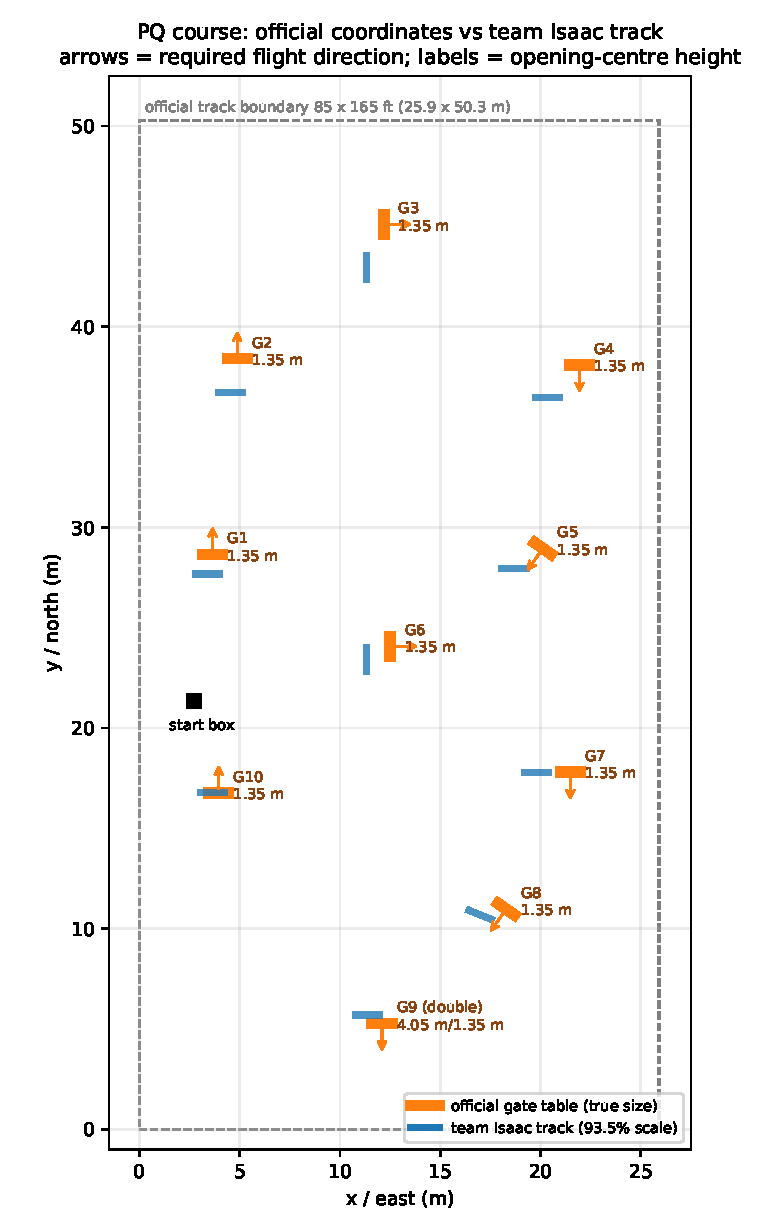
\includegraphics[height=0.62\textheight]{figs/course_overlay.pdf}
\caption{Official gate coordinates (orange, true size) against the team's Isaac track (blue). The Isaac copy is a roughly \SI{93}{\percent}-scale version of the official layout (Section~\ref{sec:track}).}
\end{figure}
\begin{table}[H]\centering\footnotesize
\begin{tabularx}{\linewidth}{@{}p{3.0cm}rrrX@{}}
\toprule
Leg & Distance & \makecell{Arrival angle\\off gate axis} & \makecell{Gate number in\\Gene's simulator} & Note \\
\midrule
start box $\rightarrow$ G1 & \SI{7.4}{m} & \SI{7}{\degree} & 6 & takeoff from the floor (never trained) \\
G1 $\rightarrow$ G2 & \SI{8.3}{m} & \SI{8}{\degree} & 7 & \\
G2 $\rightarrow$ G3 & \SI{9.0}{m} & \SI{35}{\degree} & 8 & \\
G3 $\rightarrow$ G4 & \SI{10.8}{m} & \SI{50}{\degree} & 9 & \\
G4 $\rightarrow$ G5 & \SI{7.9}{m} & \SI{22}{\degree} & 10 & G5 faces \SI{215}{\degree} \\
G5 $\rightarrow$ G6 & \SI{7.7}{m} & \textbf{\SI{152}{\degree}} & 0 & split-S (the drone passes beside G6, turns around, and comes back through it): pass north of G6, turn back east \\
G6 $\rightarrow$ G7 & \SI{9.8}{m} & \SI{50}{\degree} & 1 & \\
G7 $\rightarrow$ G8 & \SI{6.2}{m} & \SI{4}{\degree} & 2 & G8 faces \SI{215}{\degree} \\
G8 $\rightarrow$ G9 top & \SI{7.0}{m} & \SI{50}{\degree} & 3 & climb to \SI{4.05}{m}, fly south \\
G9 top $\rightarrow$ G9 bottom & turnaround & \SI{180}{\degree} & 4 & descend to \SI{1.35}{m}, fly north \\
G9 bottom $\rightarrow$ G10 & \SI{13.6}{m} & \SI{32}{\degree} & 5 & longest leg \\
G10 $\rightarrow$ G1 & \SI{10.4}{m} & \SI{2}{\degree} & 6 & lap 2 \\
\bottomrule
\end{tabularx}
\caption{Leg geometry from the official table (straight-line, plan view). Headings: the official table gives compass bearings (clockwise from north, so 215\textdegree\ points south-west); elsewhere this document uses the mathematical convention (counter-clockwise from east, so the same heading is $-$125\textdegree). A complete run is two laps; one lap is 11 crossings. Another team counts 23 crossings, finishing on gate~1.\X}
\end{table}

%======================================================================== PART II
\newpage
\part*{Part II --- Engineering journal}
\addcontentsline{toc}{part}{Part II --- Engineering journal}

\section{Project history}
\begin{table}[H]\centering\footnotesize
\begin{tabularx}{\linewidth}{@{}p{2.0cm}p{3.3cm}Xp{3.3cm}@{}}
\toprule
Dates & Branch & Approach & Outcome \\
\midrule
3 Jun & \code{main}, \code{modified-starter} & Organizer example client; HSV colour gate detection; attitude + thrust commands & controller working, untuned \\
6--16 Jun & \code{preplanning} & reactive gate chasing, then fixed waypoints & gate 1 passed \\
17--20 Jun & \code{manual-control}, \code{spline-path} & fly by keyboard to record the course, replay as a spline (VQ1 gave position data) & ``sub 14 seconds'' (commit message only) \\
28 Jun--18 Jul & \code{Qualifier2*} & VQ2 blocked state data: IMU + vision rebuild & gap analysis: ``vision not connected to flight''; abandoned \\
23--25 Jul & \code{Q2_new} & DreamerV3 (model-based RL) against the real-time simulator & 168k steps, 0 gates; deleted \\
26--27 Jul & \code{Q2_new}, \code{Q2_CV}, \code{Q2_pnp} & OpenCV and YOLO corners, PnP + IMU & passed gates 1--2 \\
28 Jul--1 Aug & \code{Q2_kalman} & dual-gate Kalman filter, tuning harness & human best 35.96\,s \\
10--30 Aug & \code{classical-vision-}\allowbreak\code{racing} & classical Li \& de Croon stack; behaviour cloning / HG-DAgger (retired as weak) & human best 14.04\,s; no autonomous lap recorded \\
\textbf{30 Aug--16 Sep} & \textbf{\code{isaacsim}} & \textbf{Isaac Lab PPO on the PQ course} & \textbf{best model \code{pq_speed_best} (5 Sep); copied into the AI\_GP repo on 16 Sep} \\
\bottomrule
\end{tabularx}
\caption{Eras of the project. The \code{isaacsim} branch contains every useful earlier branch.\V}
\end{table}

\paragraph{Where the Isaac work was done.} All 32 runs record their directory as \nolinkurl{/mnt/d/Code/Competitions/isaac_drone_racer/...}\V, a separate folder on Gene's machine. It was copied into AI\_GP on 16 Sep without its own git history. Gene reports everything relevant is pushed. Trained models for the retired VQ path are excluded from git on purpose and are not needed.

\section{Isaac training history and Gene's best model}
\begin{table}[H]\centering\small
\begin{tabularx}{\linewidth}{@{}p{2.2cm}Xp{2.2cm}p{3.6cm}@{}}
\toprule
Run & Change & Start from & Best (gates/ep, reward) \\
\midrule
30 Aug -- 2 Sep & 7- and 17-gate VQ-style tracks, observation and action redesigns, several NaN/abort runs & scratch & 1.5--4.5 gates \\
2--3 Sep & look/visibility reward experiments (policy learned to hover and stare) & scratch & $\approx$0 gates \\
3--4 Sep & zig-zag and ``passage'' shaping (\code{pass_main}, \code{vel_align}, \code{passage_shape}) & chain & 1.8--5.9 \\
4 Sep 14:49 & first PQ track (different gate order) & passage\_shape & 0.5 (transfer failed) \\
4 Sep 17:03 & PQ track, current order, gate-passed 600 & \textbf{scratch} & 25.3, 356 (\code{pq_scratch}) \\
4 Sep 20:38 & + run-in progress, velocity alignment & pq\_scratch & 30.8, 427 (\code{pq_vel}) \\
4 Sep 23:48 & run-in progress 25 & pq\_vel & 28.9, 400 (\code{pq_hook}) \\
\textbf{5 Sep 01:08} & \textbf{speed-through-gate 3.4} & pq\_hook & \textbf{33.2, 463 (\code{pq_speed_best})} \\
6 Sep 01:35 & identical settings, continued & pq\_speed\_best & \textbf{0.0 --- collapsed} (\code{pq_hook2}) \\
\bottomrule
\end{tabularx}
\caption{Training lineage (from checkpoint hashes, run configs and TensorBoard).\V\ ``Gates/ep'' is per 40\,s training episode with exploration noise.}
\end{table}

\begin{figure}[H]\centering
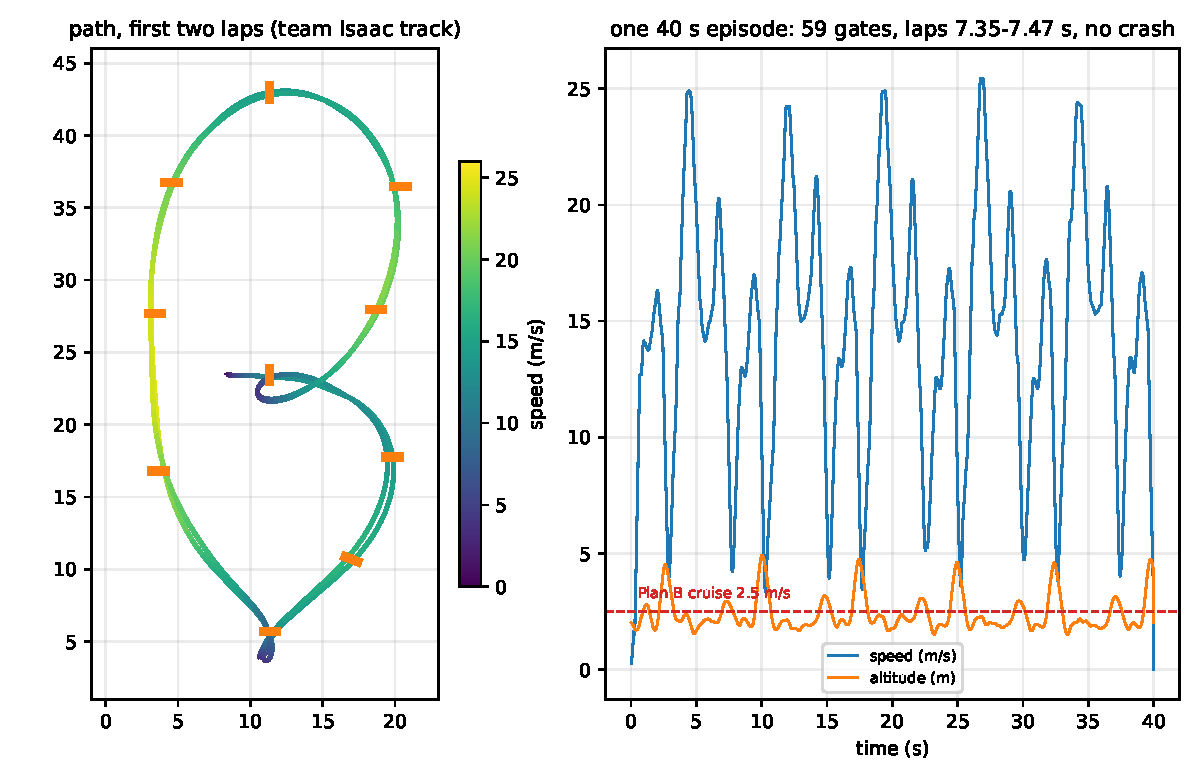
\includegraphics[width=\linewidth]{figs/keeper_play.pdf}
\caption{Gene's model flown on 16 Sep without a display, in Isaac's playback mode (fixed start position, no disturbances, and the network's single best action at every step rather than random exploration).\V\ 59 gates in 40\,s, laps 7.35--7.47\,s, mean \SI{14.4}{m/s}, peak \SI{25.4}{m/s}, altitude 1.5--4.9\,m. This reproduces the 7--8\,s lap time Gene reported from his own runs. The red dashed line marks Plan~B's gate speed for comparison.}
\end{figure}

\section{Audit findings}\label{sec:findings}

\begin{table}[H]\centering\footnotesize
\begin{tabularx}{\linewidth}{@{}p{3.3cm}XXp{2.6cm}@{}}
\toprule
Item & Gene's simulator (what the model was trained on) & Real physical qualifier & Fixed by the corrections patch? \\
\midrule
Camera view width & \SI{90}{\degree} (focal length 320\,px) & \SI{74}{\degree}--\SI{75}{\degree} (about 424\,px) & yes \\
Camera tilt & exactly \SI{20}{\degree} up & adjustable; unknown until measured & no; measure on site \\
Course size & about 93\,\% of true size & official coordinates & yes \\
Gate heights & opening centres at 2.0\,m (double gate 4.7\,m) & about 1.35\,m (double gate about 4.05\,m) & yes \\
Start & in the air, in front of gate 6 & on the floor, 7.4\,m before gate 1 & playback start only; takeoff never trained \\
Delay from camera to motors & none & roughly 50--130\,ms & no; needs training with delay \\
Stick response & straight-line mapping & Betaflight curves (nonlinear) & no; change FC settings or convert in code \\
Drag, sensor noise, bumps & none (tiny random pushes only) & present & no; needs training with them \\
Gate corners & computed exactly from the true gate position & must be found by a camera detector (none exists yet for real gates) & no \\
Which gate is next & provided by the simulator & must be counted onboard (code does not exist yet) & no \\
Communication & MAVLink over UDP & MSP over a serial cable to Betaflight & no; new code needed \\
Counting gate passes during training & broken on any reset (bug) & n/a & yes \\
\bottomrule
\end{tabularx}
\caption{Where Gene's simulator differs from the real event. The durability tests in Section~\ref{sec:stress} measure how much each difference matters.}
\end{table}


\subsection{Gate-counting bug in the current Isaac code}\label{sec:bug}
\code{tasks/drone_racer/mdp/commands.py:234}: whenever \emph{any} environment resets, \code{prev_robot_pos_w} is overwritten for \emph{all} environments. Isaac Lab~2.1 then runs the gate-crossing check in the same step (reset first, then \code{command_manager.compute}), so previous equals current and no crossing is registered anywhere.\V\ With thousands of parallel drones, resets happen almost every step. That explains why the 6 Sep continuation of Gene's model, with byte-identical settings, logged zero passes \emph{and} exactly zero misses.

\begin{minipage}{0.52\linewidth}
\begin{lstlisting}[language=Python]
# candidate fix (applied only to scratch copies)
prev = self.prev_robot_pos_w.clone()
prev[env_ids] = self.robot.data.root_pos_w[env_ids]
self.prev_robot_pos_w = prev
\end{lstlisting}
\end{minipage}\hfill
\begin{minipage}{0.45\linewidth}
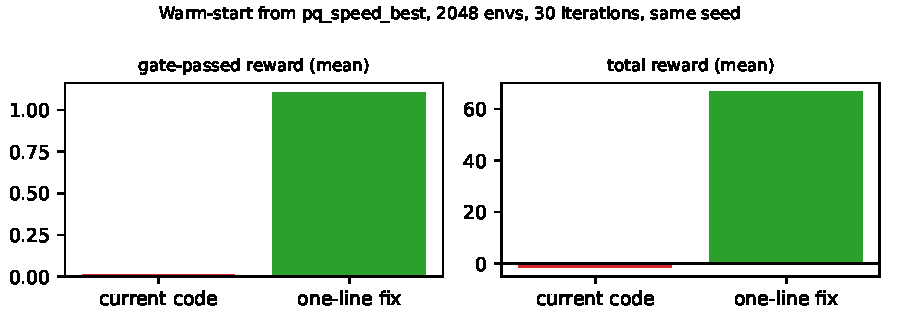
\includegraphics[width=\linewidth]{figs/bug_ab.pdf}
{\footnotesize Left: points earned for passing gates; right: total points; both averaged per training log window, before and after the fix.}
\end{minipage}

\begin{verdict}
\textbf{Confirmed by A/B test.}\V\ Starting from Gene's model with identical random seeds, the current code logs 0.014 mean gate reward and 0 misses; with the fix it logs 1.11 and 0.16. Total reward is $-1.6$ vs $+66.7$.
Any on-site retraining (which \code{PHYSICAL_TUNING.md} plans) collapses until the fix is in. Playback with one drone is mostly unaffected.
Clone before writing, because line 327 stores Isaac's buffer without copying it.
\end{verdict}

\subsection{Camera field of view: who is right?}
\begin{itemize}
\item \textbf{Code:} \code{utils/aigp_obs.py} and \code{camera_model.py} use a 640$\times$360 image with a focal length of 320 pixels (written fx\,=\,fy\,=\,320; the focal length in pixels sets how wide the view is) and a \SI{20}{\degree} upward camera tilt. That is a \SI{90.0}{\degree} horizontal FOV, taken from the \emph{VQ} simulator spec.\V
\item \textbf{PQ spec} (VADR-TS-005 \S3.8): \SI{75}{\degree} horizontal FOV at 1920$\times$1080.
\item \textbf{Measurement}\X: AI of Sauron calibrated the same camera model with a ChArUco board, on their own lens: fx\,=\,1270.7\,px, fy\,=\,1267\,px, principal point (976, 497), five distortion coefficients, and 0.28\,px reprojection error. That is \SI{74.1}{\degree}$\times$\SI{46.2}{\degree}.
\end{itemize}
\begin{figure}[H]\centering
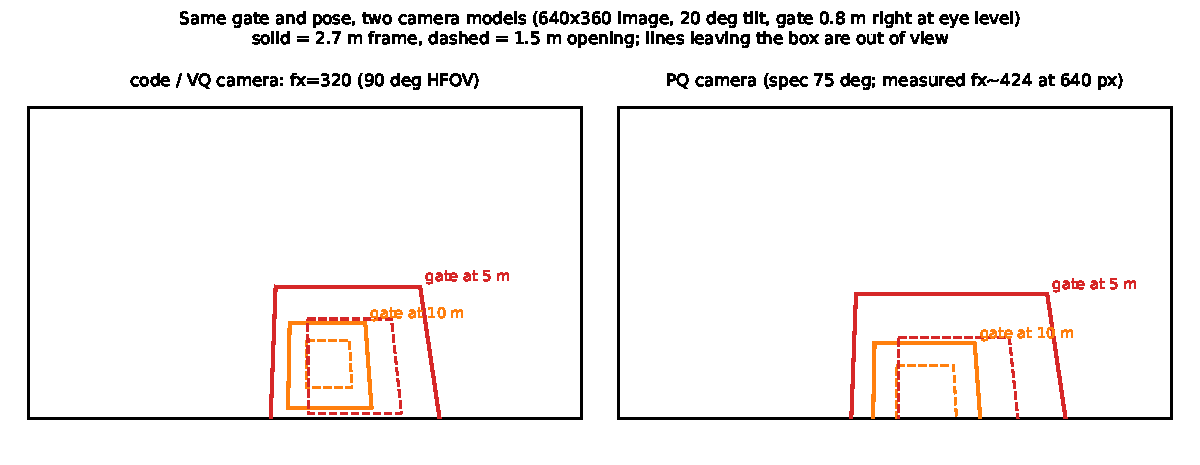
\includegraphics[width=\linewidth]{figs/camera_fov.pdf}
\caption{The same gate rendered with the code's camera and with the PQ camera. Gates appear about 32\,\% larger and farther off-centre on the real camera, which is exactly the input the policy normalises.}
\end{figure}
\begin{verdict}
\textbf{Our code is wrong for the PQ; the spec and the measurement agree.}
The specification is the authority and it says \SI{75}{\degree} horizontal, which at 640\,px width is a focal length of \textbf{417.0\,px}, not 320. (The corrections patch of 16 Sep used 423.6\,px, i.e.\ \SI{74.1}{\degree}, taken from another team's calibration of their own lens; \textbf{use 417.0} until we calibrate ours.) The real principal point also sits about 14\,px above centre, and the lens distortion is significant.
A \SI{74}{\degree} image cannot be remapped to \SI{90}{\degree}, so the policy must either be retrained with the real intrinsics or shown to tolerate the change (Section~\ref{sec:stress}).
Camera tilt on our drones is still unmeasured. Calibrate on day~1; it takes about 15 minutes.
\end{verdict}

\subsection{Track size and gate heights: who is right?}\label{sec:track}
The Isaac track comment says it was digitized by assuming the pylons are \SI{15}{m} apart. We fitted the 11 Isaac gate centres to the organizer's numeric gate table with a similarity transform (scale, rotation, translation):
\begin{itemize}
\item best fit: \textbf{scale 0.9348}, rotation \SI{0.03}{\degree}, all gates within \SI{0.42}{m};
\item forcing scale $=1$ leaves errors up to \SI{1.47}{m}.\V
\end{itemize}
Headings agree except gate~5 (Isaac \SI{-90}{\degree} vs official \SI{-125}{\degree}, off by \SI{35}{\degree}) and gate~8 (off by \SI{13}{\degree}).
The official boundary, $85\times165$\,ft $=25.9\times50.3$\,m, also matches the ``$25.9\times50.3$\,m'' label on the spec plan.
\begin{verdict}
\textbf{The Isaac track is \SI{6.5}{\percent} too small, and two gate headings are off.} The organizer table is numeric; the Isaac copy was measured off a picture with an assumed ruler.
\textbf{Heights:} Isaac places opening centres at \SI{2.0}{m} (double gate \SI{4.7}{m}). Floor-standing 2.7\,m frames put them at \SI{1.35}{m} (double gate \SI{4.05}{m}), as confirmed on site by another team.\X
\textbf{Start:} Gene's simulator numbers the gates starting from the centre gate (official gate~6 is its gate~0), and its playback mode starts in the air in front of that gate. The real race starts on the floor, 7.4\,m before official gate~1, which is gate~6 in Gene's numbering.
Confirm with a tape measure on day~1: one gate-to-gate distance settles the scale.
\end{verdict}
\begin{warnbox}[Unresolved as of 17 September: the hall footprint]
The specification (\S3.4) states the track footprint is \textbf{\SI{60}{m}\,$\times$\,\SI{21}{m}}. The plan drawing, measured with its own printed ruler, gives \textbf{\SI{25.9}{m}\,$\times$\,\SI{50.25}{m}}. Those do not reconcile by any single scale factor --- the spec's track is \emph{longer} and \emph{narrower}. Most likely the spec quotes the usable hall volume and the drawing quotes the gate envelope, but that is a guess. \textbf{The on-site survey settles it, and until it does, no document should be trusted for absolute course size.}
\end{warnbox}

Clarification on drone mass: the \emph{simulated} drone's mass does not differ from the mass its own thrust model assumes --- both are \SI{0.6076}{kg}.\V\ There is no internal mismatch. The real drone weighs \SI{1745}{g}, which is a different problem entirely and is explained in the status section at the front of this document.

\subsection{Flight-controller configuration}
From another team's full \code{dump all} of the same drone model\X:
\begin{itemize}
\item \textbf{Firmware and modes:} Betaflight 4.4.3 (H743). ARM is on AUX1 (pilot's CRSF radio) and \textbf{MSP OVERRIDE} is on AUX5. No ANGLE/HORIZON mode is assigned, so it flies ACRO.
\item \textbf{Override mask:} \code{msp_override_channels_mask = 11}, i.e.\ roll, pitch and yaw only. \textbf{Throttle is not overridden}; autonomy needs 15.
\item \textbf{Rates:} Betaflight rates with rc\_rate 0.55 and super\_rate 0.75, about \SI{440}{\degree\per\second} at full stick and \textbf{nonlinear}. The policy assumes linear $\pm$\SI{183}{\degree\per\second}.
\item \textbf{Throttle curve:} \code{thr_mid 54}, \code{thr_expo 68}, \textbf{nonlinear}. The plant assumes linear.
\item \textbf{Failsafe:} \code{failsafe_procedure = DROP}.
\item \textbf{Units:} MSP raw gyro is in counts (16.4 per \si{\degree\per\second}), not \si{\degree\per\second}.
\end{itemize}
\begin{warnbox}[Safety fact from the Betaflight 4.4.3 source]
In \code{src/main/rx/msp_override.c}, while the override switch is on, the FC uses the \textbf{last} \code{MSP_SET_RAW_RC} values it received, \textbf{with no timeout}.\X\ If the Jetson process hangs mid-flight, the drone keeps flying its last command until the pilot flips the switch off or disarms.
Stream a safe neutral frame before enabling override, run a separate stall watchdog, and brief the pilot.
\end{warnbox}

\subsection{The missing deployment layer}\label{sec:missing}
\begin{warnbox}[This is the critical path, confirmed 17 September]
A repo-wide search finds no occurrence of MSP anywhere in the flight client.\V\ \code{controller.py} sends MAVLink \code{SET_ATTITUDE_TARGET} to a \code{sim_conn} --- the virtual qualifier's simulator interface. Betaflight does not accept MAVLink attitude setpoints, and the PQ specification confirms the real interface is \textbf{MSP over UART}. \textbf{Nothing we have can currently send a single command to the real drone.} Every other activity that involves flying is downstream of fixing this.
\end{warnbox}
A repo-wide search also finds no occurrence of serial, Betaflight, Jetson, TensorRT, GStreamer/Argus or CLOCK\_MONOTONIC in the client.\V\ To fly anything on the real drone we need:
\begin{enumerate}
\item an MSP bridge (commands out; attitude, raw IMU, status and battery in);
\item Jetson camera capture with capture timestamps;
\item a gate detector that works on \emph{real} gate images (the existing detectors were tuned on simulator images);
\item an onboard gate/lap counter, because the policy's ``next gate number'' input came from the simulator and both learned planners raise an error without it;\V
\item real-drone safety: crash detection, arming, finish and landing. The existing logic is simulator-based and auto re-arms after a crash.\V
\end{enumerate}
Both Plan~A and Plan~B need items 1, 2, 3 and 5.

\subsection{Smaller items}
\begin{itemize}
\item \textbf{Parity tests:} the two AI\_GP$\leftrightarrow$Isaac observation parity tests silently skip after vendoring (path moved). With the path fixed, all 29 pass.\V
\item \textbf{Bridge defaults:} the bridge's default weights path points to a VQ-era file; use \code{pq_speed_best.pt} explicitly. It also enables a ``visual snap'' history rewrite that training never used.\V
\item \textbf{Stale scripts:} \code{scripts/rl/probe_race.py} references a removed reward term and will crash.\I
\end{itemize}

%------------------------------------------------------------------------
\section{Durability study (16 Sep)}\label{sec:stress}
\subsection{Method}
\begin{itemize}
\item \textbf{Setup:} each test (``scenario'') runs Gene's model, always taking its single best action, on 512 simulated drones at once for 40\,s (2400 control steps); tests run later in the day used 20\,s.
\begin{itemize}
\item Each simulated drone flies until it crashes, is immediately reset, and tries again. One start-to-crash flight is an \emph{attempt}.
\item Unless a row says ``race start'', each attempt begins just past a randomly chosen gate, as in training. ``Race start'' means every attempt begins in front of official gate~1, like the real race.
\item Every test uses a copy of Gene's code with the gate-counting bug fixed. The changes being tested are applied at runtime; none of the team's files were modified.
\end{itemize}
\end{itemize}

\begin{explain}[How to read the numbers in the tables below]
\begin{itemize}
\item \textbf{Gates per attempt:} how many gates a drone gets through, on average, before it crashes. Higher is better. In the 20--40\,s tests a good model is capped by the test length (about 20--28).
\item \textbf{Crashes per 100 gates:} total crashes divided by total gates passed, times 100. A crash is hitting anything (including the floor), crossing a gate's plane outside its opening, or flying more than 20\,m away from the next gate. Crashes in the first 1.5\,s after a random start are ignored. Lower is better.
\begin{itemize}
\item This is \emph{not} a percentage, so it can exceed 100. A value of 110 means the drone usually crashes before it passes even one gate.
\end{itemize}
\item \textbf{Chance of two clean laps} (written $P$(2 laps)): the probability of passing the 22 gate crossings of two laps (11 per lap, the double gate counting twice) without a single crash, estimated as $\max(0,\,1-\text{crashes per gate})^{22}$. It is 0\,\% whenever crashes outnumber gates.
\item \textbf{Test length:} 40\,s for the first tests, 20\,s for tests run later in the day, 25\,s for the retraining comparison. Crashes per 100 gates can be compared across lengths; gates per attempt only within the same length.
\item \textbf{Test labels:} codes such as ``A6'' or ``S1'' are just short names for individual tests. Their meaning is written out in each row.
\item \textbf{Realism levels} (the ``Band'' column):
\begin{itemize}
\item \textbf{Reference:} Gene's own simulated course, as trained.
\item \textbf{Expected:} things that will almost certainly be true at the real event:
\begin{itemize}
\item the true course size and gate heights;
\item the real camera;
\item gates placed a little off the map;
\item imperfect gate detection;
\item about 50\,ms of delay between seeing and acting;
\item a hover thrust that is slightly wrong;
\item a heavier, slower-responding 8-inch drone;
\item air drag.
\end{itemize}
There is no wind, because the event is indoors.
\item \textbf{Rougher:} plausible but pessimistic versions of the same things, plus small bumps (propeller wash, a light touch).
\item \textbf{Stress only:} things not expected at the event: wind, hard bumps, 200\,ms delay, resized gates, and completely different courses. The last group tests whether the model memorized the course rather than learning to fly.
\item \textbf{Combined:} rows marked ``combined'' apply all the disturbances of their level at once.
\end{itemize}
\end{itemize}
\end{explain}

\subsection{Results}
\IfFileExists{stress_table.tex}{{\footnotesize\setlength{\tabcolsep}{3pt}
\begin{longtable}{@{}p{1.5cm} p{5.3cm} r r r r r r@{}}
\toprule
Realism level & Test & \makecell{Gates per\\attempt} & \makecell{Crashes /\\100 gates} & \makecell{$P$(2 laps,\\no crash)} & \makecell{Median\\lap (s)} & \makecell{Speed at\\gate (m/s)} & \makecell{Lateral\\offset p95 (m)} \\
\midrule\endhead
Reference & \textbf{R0} baseline (Gene's course, small random pushes as in training) & 21.9 & 2.6 & 56\,\% & 7.43 & 15.98 & 0.466 \\
Reference & \textbf{R1} ideal (Gene's course, no pushes) & 27.8 & 1.7 & 69\,\% & 7.43 & 16.03 & 0.465 \\
Expected & \textbf{A1} official course: true size and floor-standing gates & 7.9 & 9.9 & 10\,\% & 8.07 & 15.73 & 0.494 \\
Expected & \textbf{A1b} official size, Gene's gate heights & 8.0 & 9.8 & 10\,\% & 8.07 & 15.71 & 0.492 \\
Expected & \textbf{A1c} Gene's size, floor-standing gate heights & 26.5 & 1.8 & 67\,\% & 7.43 & 16.03 & 0.465 \\
Expected & \textbf{A2} real camera: 74\textdegree field of view & 1.1 & 42.4 & 0\,\% & -- & 13.96 & 0.558 \\
Expected & \textbf{A3} camera tilt 15\textdegree (-5) & 1.9 & 32.1 & 0\,\% & 7.85 & 13.52 & 0.582 \\
Expected & \textbf{A4} gate placement $\pm$0.25 m, $\pm$5\textdegree & 9.5 & 6.3 & 24\,\% & 7.52 & 15.88 & 0.49 \\
Expected & \textbf{A5} gate-detection noise 2 px, 5\% missed frames & 9.8 & 5.4 & 30\,\% & 7.52 & 15.73 & 0.48 \\
Expected & \textbf{A6} latency 50 ms (vision 33 + command 17) & 0.6 & 55.2 & 0\,\% & -- & 14.53 & 0.592 \\
Expected & \textbf{A7} thrust calibration -10\% & 1.0 & 57.7 & 0\,\% & -- & 14.03 & 0.567 \\
Expected & \textbf{A8} slower airframe (response lag 40 ms) & 6.9 & 9.7 & 11\,\% & 7.52 & 16.44 & 0.507 \\
Expected & \textbf{A10} 8-inch drone clearance (must pass within 1.1 m box) & 14.0 & 2.9 & 52\,\% & 7.43 & 16.06 & 0.467 \\
Rougher & \textbf{B1} gate placement $\pm$0.5 m, $\pm$10\textdegree, $\pm$0.2 m z & 5.1 & 14.5 & 3\,\% & 7.65 & 15.73 & 0.514 \\
Rougher & \textbf{B2} gate-detection noise 5 px, 15\% missed, 5\% corners & 2.0 & 26.9 & 0\,\% & 7.96 & 14.91 & 0.546 \\
Rougher & \textbf{B3} latency 100 ms & 0.1 & 94.7 & 0\,\% & -- & 9.52 & 0.446 \\
Rougher & \textbf{B6} gate detection only 15 times per second & 5.1 & 13.0 & 5\,\% & 7.71 & 15.95 & 0.522 \\
Rougher & \textbf{B7} small bumps (every ~3 s) & 14.8 & 2.8 & 53\,\% & 7.43 & 16.06 & 0.472 \\
Stress only & \textbf{C4} gates 20\% smaller & 5.9 & 11.3 & 7\,\% & 7.6 & 15.72 & 0.413 \\
Stress only & \textbf{C5} mirrored course & 0.7 & 73.4 & 0\,\% & -- & 15.29 & 0.53 \\
Stress only & \textbf{C7} random course & 0.7 & 46.9 & 0\,\% & -- & 13.02 & 0.564 \\
\bottomrule
\caption{Durability results for Gene's model (\code{pq_speed_best}). 512 simulated drones per row; the model always takes its single best action; the gate-counting bug is fixed. Tests R0--A3 ran for 40\,s and the rest for 20\,s, which also caps their gates per attempt. How to read the columns: see the box above. Speed at gate: average speed while passing through a gate. Lateral offset p95: in 95\,\% of passes, the drone's centre was at most this far sideways from the centre of the 1.5\,m opening (0.75\,m would be touching the edge).}\label{tab:stress}
\end{longtable}}
}{\textit{(results pending)}}
\IfFileExists{figs/stress_results.pdf}{\begin{figure}[H]\centering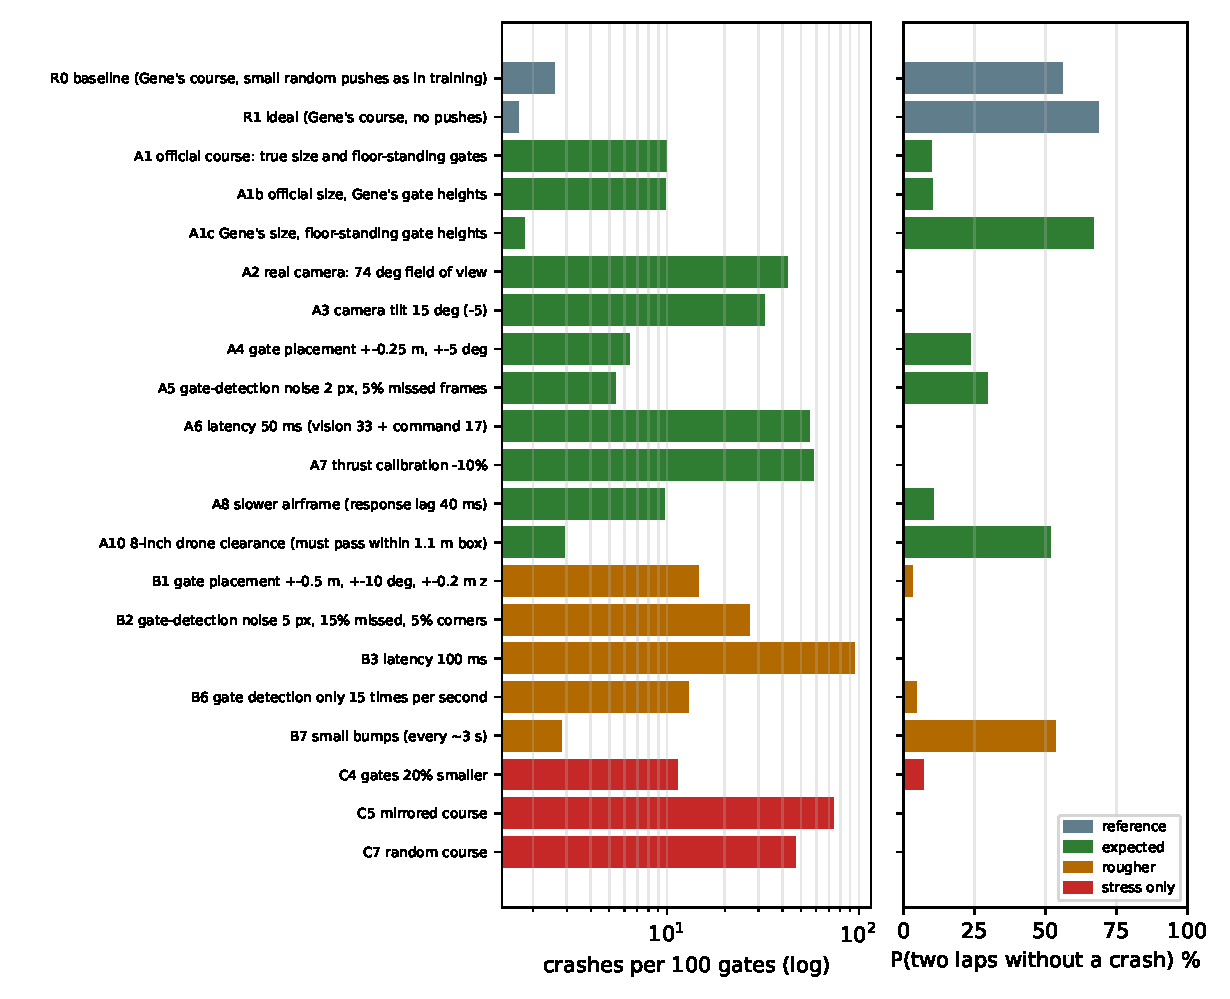
\includegraphics[width=\linewidth]{figs/stress_results.pdf}\caption{Crash rate per 100 gates (log scale) and the implied chance of finishing two laps, by scenario and realism band.}\end{figure}}{}
\IfFileExists{stress_discussion.tex}{
\begin{table}[H]\centering\footnotesize
\begin{tabularx}{\linewidth}{@{}Xrr@{}}
\toprule
One change at a time to Gene's model on Gene's own course (unchanged: 2 crashes per 100 gates) & \makecell{Crashes /\\100 gates} & $P$(2 laps) \\
\midrule
Thrust calibration $-$10\,\% & 58 & 0\,\% \\
Latency 50\,ms & 55 & 0\,\% \\
Real camera (fx 424) & 42 & 0\,\% \\
Camera tilt $-$\SI{5}{\degree} & 32 & 0\,\% \\
Spec drawing exactly (Gene's heights) & 16 & 2\,\% \\
Scale only (Gene's map $\times$1.075) & 16 & 2\,\% \\
Gates 20\,\% smaller & 11 & 7\,\% \\
True course size & 10 & 10\,\% \\
Slower airframe (40\,ms) & 10 & 11\,\% \\
Gate placement $\pm$0.25\,m & 6 & 24\,\% \\
Detector noise 2\,px & 5 & 30\,\% \\
8-inch clearance & 3 & 52\,\% \\
Correct gate heights only & 2 & 67\,\% \\
\midrule
Latency 100\,ms (rougher) & 95 & 0\,\% \\
Vision 15\,Hz (rougher) & 13 & 5\,\% \\
Detector noise 5\,px, 15\,\% missed (rougher) & 27 & 0\,\% \\
Small bumps (rougher) & 3 & 53\,\% \\
Gate placement $\pm$0.5\,m (rougher) & 15 & 3\,\% \\
\midrule
Mirror-image course (stress only) & 73 & 0\,\% \\
Randomly generated course (stress only) & 47 & 0\,\% \\
\bottomrule
\end{tabularx}
\caption{The sensitivity of Gene's model to single realistic factors, ranked.}\label{tab:sens}
\end{table}

\begin{verdict}[What the durability tests say about Gene's model]
\begin{itemize}
\item \textbf{Most damaging factors:} latency and thrust calibration. Just \textbf{50\,ms} of total delay (55 crashes per 100 gates), or a hover thrust \textbf{10\,\% weaker} than assumed (58), is enough to make two laps essentially impossible. The real Jetson$\rightarrow$MSP$\rightarrow$Betaflight path will have at least that much delay (another team budgets about 130\,ms), and hover thrust will only be known after measurement.
\item \textbf{Camera model:} the real field of view (42) and a \SI{5}{\degree} tilt error (32) are next.
\item \textbf{Course geometry:} scaling Gene's own map up by 7.5\,\%, with nothing else changed, raises crashes from 2 to 16 per 100 gates. About 60\,\% of those crashes are on the climb to the \emph{upper opening of the double gate}: the policy learned a manoeuvre timed to the exact distances it trained on. Heights alone do not matter (2).
\item \textbf{Mild factors:} gate placement ($\pm$0.25\,m), detector noise (2\,px) and the larger 8-inch airframe are comparatively mild, at 6, 5 and 3 crashes per 100 gates.
\item \textbf{It memorized this course.} On a mirrored or random course it crashes almost immediately (73 and 47). That is expected: its input includes ``which gate is next'', so it learns the course, not a general skill. This is fine for a fixed course only if every other detail of the course and the drone matches training.
\item \textbf{Is the 7--8\,s lap time itself the problem?} Not directly; the speed is a symptom. The real problem is a policy optimized for an idealized plant with zero latency, exact thrust, and a camera and course that differ from reality. A retrain needs randomization of exactly the top factors above: latency (0--150\,ms), thrust scale ($\pm$15\,\%), camera tilt ($\pm$\SI{5}{\degree}), rate lag. It also needs the corrected camera and course (Section~\ref{sec:retrain}).
\end{itemize}
\end{verdict}
}{}

\subsection{Retraining on the corrected simulator (16 Sep)}\label{sec:retrain}
\textbf{Setup.} As a feasibility test, Gene's model was trained further (fine-tuned) for one hour on bojro's laptop in a corrected copy of the simulator (the \code{pq_corrections.patch} changes):
\begin{itemize}
\item \textbf{Corrections:} official track and heights, the \SI{74}{\degree} camera, and the gate-counting fix.
\item \textbf{Randomized ``expected'' disturbances}, so the model sees them during training:
\begin{itemize}
\item 33\,ms vision and 17\,ms command latency;
\item 2\,px keypoint noise with 5\,\% missed frames;
\item attitude and gyro noise;
\item a 30\,ms rate lag and drag;
\item a per-drone thrust scale of $\pm$10\,\%;
\item per-drone gate shifts of $\pm$0.25\,m and $\pm$\SI{5}{\degree}.
\end{itemize}
\item \textbf{Size:} 2048 drones, 32.4k PPO timesteps (about 66M samples), roughly $\frac{1}{3}$ of one of Gene's standard 50k-step, 4096-drone fine-tunes.
\end{itemize}
\IfFileExists{figs/retrain_curves.pdf}{\begin{figure}[H]\centering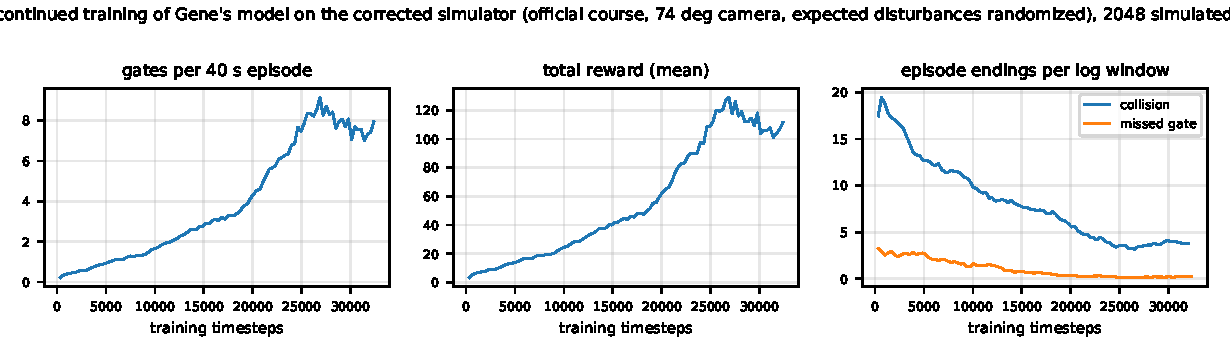
\includegraphics[width=\linewidth]{figs/retrain_curves.pdf}\caption{Training curves of the one-hour fine-tune.}\end{figure}}{}
\IfFileExists{retrain_table.tex}{\begin{table}[H]\centering\footnotesize
\begin{tabularx}{\linewidth}{@{}Xrrrr@{}}
\toprule
Test on the corrected simulator & \makecell{Gates per\\attempt} & \makecell{Crashes /\\100 gates} & \makecell{$P$(2 laps,\\no crash)} & \makecell{Median\\lap (s)} \\
\midrule
No disturbances -- Gene's model & 0.9 & 51.4 & 0\,\% & -- \\
Expected disturbances -- Gene's model & 0.3 & 110.3 & 0\,\% & -- \\
Expected disturbances, race start -- Gene's model & 0.6 & 70.3 & 0\,\% & -- \\
Rougher disturbances -- Gene's model & 0.1 & 302.7 & 0\,\% & -- \\
No disturbances -- 1-hour retrain & 1.2 & 59.7 & 0\,\% & -- \\
Expected disturbances -- 1-hour retrain & 6.3 & 11.2 & 7\,\% & 11.01 \\
Expected disturbances, race start -- 1-hour retrain & 4.7 & 11.8 & 6\,\% & 10.95 \\
Rougher disturbances -- 1-hour retrain & 0.3 & 134.2 & 0\,\% & -- \\
\bottomrule
\end{tabularx}
\caption{Gene's model vs the 1-hour retrain on the corrected simulator: official course and real \SI{74}{\degree} camera (512 drones, 25\,s each). ``Race start'' means every attempt starts in front of official gate~1. ``Expected'' and ``rougher'' apply all disturbances of that realism level at once (Section~\ref{sec:stress}). Gates per attempt counts every start-to-crash attempt; a crash rate above 100 means most attempts crash before passing a single gate.}\label{tab:retrain}
\end{table}
\begin{itemize}
\item Clean playback from official gate~1, Gene's model: 11$\times$ 4 gates then collision; laps: no complete lap.
\item Clean playback from official gate~1, the 1-hour retrain: 15$\times$ 2 gates then collision; laps: no complete lap.
\end{itemize}
}{\textit{(evaluation pending)}}
\IfFileExists{retrain_discussion.tex}{\begin{verdict}[What the retraining test shows]
\begin{itemize}
\item \textbf{Gene's model does not survive the corrections.} On the corrected simulator (official course and real camera), it gets through only 0.1--0.9 gates per attempt: 51 to 303 crashes per 100 gates. In a clean playback run starting at official gate~1, it passes 4 gates and crashes, every time. With the real camera and course, expect it to crash within the first few gates.
\item \textbf{One hour of further training helps a lot, but only under the conditions it trained on.} With the expected disturbances:
\begin{itemize}
\item the retrained model gets through 6.3 gates per attempt, with 11 crashes per 100 gates. Gene's model gets 0.3 and 110, so this is about 10$\times$ better;
\item when it completes a lap, the lap takes about 11\,s, slower than Gene's 7.4\,s laps in his original simulator.
\end{itemize}
\item \textbf{It is not yet reliable, and it only works in a narrow range.}
\begin{itemize}
\item Only 6--7\,\% of runs would complete two laps.
\item It does worse with \emph{no} disturbances at all, because it learned to expect delay and drag.
\item It still fails under rougher disturbances.
\item A clean playback run crashes after 2 gates.
\end{itemize}
\item \textbf{Conclusion:} training on the corrected simulator is the right direction, but it needs several hours rather than one. It also needs the disturbances varied over wide ranges (camera tilt, delay, drag, detection noise), so that it copes with both calm and rough conditions, and every candidate must be checked with these tests before flying. Until a retrained model passes the Sunday go/no-go check on the real drone, Plan~B is the plan for scoring.
\end{itemize}
\end{verdict}
}{}

\subsection{How long proper retraining takes on bojro's laptop}
\begin{table}[H]\centering\small
\begin{tabular}{@{}lr@{}}
\toprule
Job (RTX 4060 Laptop, WSL, 2048 drones, measured $\approx$9.3--10 timesteps/s $\approx$ 20k samples/s) & Time \\
\midrule
One-hour feasibility fine-tune above (32.4k timesteps) & 55--60\,min \\
Standard 50k-timestep fine-tune (2048 drones) & $\approx$1\,h\,25\,min \\
Same samples as Gene's 50k-timestep, 4096-drone runs (205M samples) & $\approx$2\,h\,50\,min \\
Gene's model's entire training history, from scratch (634M samples) & $\approx$8\,h\,45\,min \\
\bottomrule
\end{tabular}
\caption{Projected training times.}
\end{table}
\textbf{Constraints and caveats:}
\begin{itemize}
\item \textbf{GPU memory:} 8\,GB fits one Isaac job at a time (training uses 5.5\,GB).
\item \textbf{RAM:} WSL is capped at 7.5\,GB and training uses 4.7\,GB. 4096 drones would need a bigger WSL memory cap (a WSL restart) and might not fit in GPU memory.
\item \textbf{CPU:} throughput is limited by the CPU/Python loop (the GPU sits near 52\,\%), so other CPU jobs slow training noticeably.
\item \textbf{Power:} keep the laptop on AC and awake.
\end{itemize}
Gene's RTX 4070 Laptop is of the same order per step.


%------------------------------------------------------------------------
\section{Plan A and Plan B}
\begin{table}[H]\centering\small
\begin{tabularx}{\linewidth}{@{}lXX@{}}
\toprule
& Plan A (existing policy) & Plan B (moderate, deterministic) \\
\midrule
Brain & \code{pq_speed_best} PPO & state machine: fly to an approach point, face, align on the gate, creep, punch through \\
FC mode & ACRO (Jetson sends body rates) & ANGLE (FC self-levels; Jetson sends angles + throttle) \\
Speed & $\approx$\SI{14}{m/s} mean, \SI{25}{m/s} peaks; 7.4\,s laps in Gene's simulator & through gates at \SI{2.5}{m/s}, up to \SI{4}{m/s} between gates; $\approx$2:05 for two laps in simulation (``balanced'' setting) \\
Needs & MSP bridge, real-image keypoints matching training, linear rate/throttle curves, gate counter; probably a retrain with real intrinsics and track & MSP bridge, gate detector tuned on real frames, hover throttle, pitch$\rightarrow$speed calibration, FC mode change (ask first) \\
Risk & high (sim-to-real gap at speed) & low \\
\bottomrule
\end{tabularx}
\caption{The two plans share the same foundation: MSP link, camera capture, logging, bench checks.}
\end{table}

\subsection{Plan B speed budget}
\begin{itemize}
\item \textbf{Why not crawl:} too slow risks an unknown run-time limit (VQ capped runs at 8\,min), eats 15-minute slots, drains the battery while hovering, and accumulates drift between gate sightings.
\item \textbf{Why not faster:} above about \SI{4}{m/s}, a look-and-servo controller runs out of turning radius and latency margin.
\end{itemize}
\begin{table}[H]\centering\small
\begin{tabular}{@{}lrrrrrl@{}}
\toprule
Tier & Cruise & Tightest turn (\SI{20}{\degree} bank) & Stop distance & Latency travel (100\,ms) & Lap & 2-lap run \\
\midrule
slow & \SI{1.5}{m/s} & \SI{0.6}{m} & \SI{0.4}{m} & \SI{15}{cm} & $\approx$120\,s & $\approx$4.3\,min \\
\textbf{medium} & \textbf{\SI{2.5}{m/s}} & \SI{1.8}{m} & \SI{1.2}{m} & \SI{25}{cm} & $\approx$75\,s & $\approx$\textbf{2.9\,min} \\
quick & \SI{3.5}{m/s} & \SI{3.4}{m} & \SI{2.3}{m} & \SI{35}{cm} & $\approx$57\,s & $\approx$2.2\,min \\
(too fast) & \SI{5.0}{m/s} & \SI{7.0}{m} & \SI{4.8}{m} & \SI{50}{cm} & & \\
\bottomrule
\end{tabular}
\caption{Plan B speed limits: back-of-envelope physics for flying \emph{through a gate} at each speed. Between gates the drone may go faster, because it slows down before each gate. In the simulation these became the settings ``safe'', ``balanced'' and ``fast'' (Table~\ref{tab:planb}; the simulation in Section~\ref{sec:planbsim} supersedes the lap estimates). Clearance inside the 1.5\,m opening is about $\pm$\SI{0.45}{m} for a roughly \SI{0.6}{m} airframe (measure ours).}
\end{table}
\begin{itemize}
\item \textbf{Speed control without a velocity sensor:} in ANGLE mode, speed settles where $v \approx g\tan(\text{pitch})/k$. Calibrate pitch$\rightarrow$speed from one logged straight flight, close the loop on the gate's apparent growth (range rate), and cap pitch at \SI{12}{\degree}.
\item \textbf{Anti-stall rules:} alignment is time-boxed to 1.5\,s; a lost gate gets one search sweep, after which the drone slows down rather than aborting; each leg has a time budget of $2\times$ its expected duration.
\end{itemize}

\begin{figure}[H]\centering
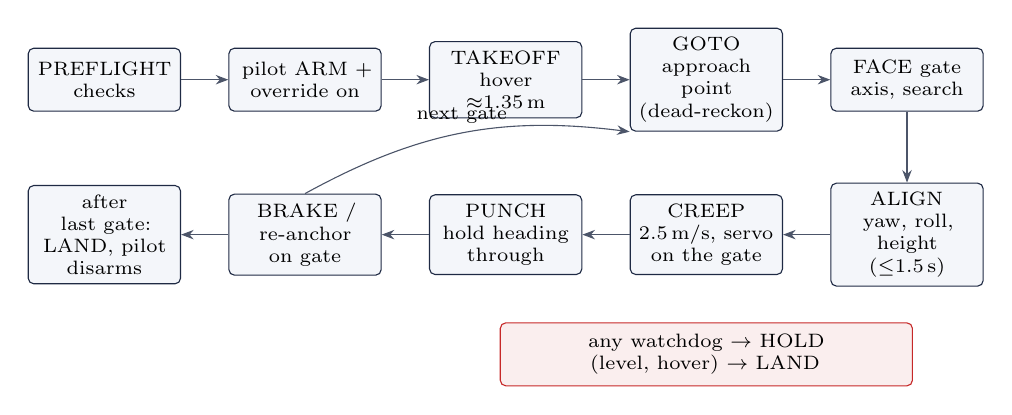
\begin{tikzpicture}[node distance=4mm and 6mm,
  st/.style={draw=ink,rounded corners=2pt,fill=soft,font=\scriptsize,align=center,minimum height=8mm,text width=17mm},
  bad/.style={st,fill=badred!8,draw=badred},
  arr/.style={-{Stealth[length=1.6mm]},draw=ink!80}]
\node[st] (pre) {PREFLIGHT\\checks};
\node[st,right=of pre] (arm) {pilot ARM +\\override on};
\node[st,right=of arm] (to) {TAKEOFF\\hover $\approx$1.35\,m};
\node[st,right=of to] (goto) {GOTO\\approach point\\(dead-reckon)};
\node[st,right=of goto] (face) {FACE gate\\axis, search};
\node[st,below=9mm of face] (align) {ALIGN\\yaw, roll, height\\($\le$1.5\,s)};
\node[st,left=of align] (creep) {CREEP\\\SI{2.5}{m/s}, servo\\on the gate};
\node[st,left=of creep] (punch) {PUNCH\\hold heading\\through};
\node[st,left=of punch] (brake) {BRAKE /\\re-anchor on gate};
\node[st,left=of brake] (land) {after last gate:\\LAND, pilot disarms};
\node[bad,below=6mm of creep,text width=50mm] (hold) {any watchdog $\rightarrow$ HOLD (level, hover) $\rightarrow$ LAND};
\draw[arr] (pre)--(arm); \draw[arr] (arm)--(to); \draw[arr] (to)--(goto); \draw[arr] (goto)--(face);
\draw[arr] (face)--(align); \draw[arr] (align)--(creep); \draw[arr] (creep)--(punch); \draw[arr] (punch)--(brake);
\draw[arr] (brake.north) to[bend left=18] node[above,font=\scriptsize]{next gate} (goto.south west);
\draw[arr] (brake)--(land);
\end{tikzpicture}
\caption{Plan B state machine. Special moves: at the G6 split-S, pass north of the gate and turn back east; at G9, top opening southbound, descend, then bottom opening northbound.}
\end{figure}
\IfFileExists{planb_section.tex}{
\subsection{Plan B tested in simulation (16 Sep)}\label{sec:planbsim}
Plan B was implemented and tested in a purpose-built CPU simulator (\code{~/aigp/tools/planb_sim.py}), run in parallel while the GPU was busy with Isaac. It is lower fidelity than Isaac, but it models the things that decide whether Plan B can work.

\textbf{What the simulator models:}
\begin{itemize}
\item \textbf{Airframe:} a simplified drone (a point with mass) flying in Betaflight's self-levelling ANGLE mode, with first-order attitude, yaw-rate and thrust lags; linear drag; per-run thrust-calibration error; random bumps (rougher conditions only).
\item \textbf{Course:} the official layout, two laps plus the finishing pass through gate~1 (23 gate crossings; the double gate counts twice per lap), with every gate shifted per run away from the map.
\item \textbf{Vision:} the real \SI{74}{\degree}$\times$\SI{46}{\degree} camera, tilted \SI{10}{\degree} up. Plan~B flies slowly with little forward lean, so it uses a smaller tilt than the \SI{20}{\degree} in Gene's simulator; the tilt is adjustable on the drone. Whenever the next gate is in view at 1.2--14\,m, the camera gives a position and heading measurement relative to that gate. That measurement has noise that grows with distance, occasional dropouts, and a delay.
\item \textbf{Between camera measurements:} the drone estimates its motion from its tilt, its thrust and an air-drag estimate (off by up to $\pm$10\,\% in expected conditions and $\pm$30\,\% in rougher ones). Height comes from the flight controller's barometer (air-pressure altimeter), whose drift is corrected by the camera. Heading slowly drifts, and the tilt reading has a small error.
\item \textbf{Scoring on the true state:} a pass requires the airframe (\SI{0.3}{m} half-span, \SI{0.12}{m} half-height) to clear the 1.5\,m opening. Touching any frame, the floor or the boundary, or missing a gate, ends the run.
\end{itemize}

\textbf{The controller} is the Plan B state machine:
\begin{itemize}
\item \textbf{Takeoff:} a staged throttle ramp.
\item \textbf{Approach:} point the camera at the gate, and commit only when height and lateral offset are lined up. Commitment is time-boxed, with fallbacks at 1.5\,s, 4\,s and 8\,s.
\item \textbf{Pass:} fly along the gate axis.
\item \textbf{G6 split-S:} bypass with the camera on G6, then stop on the far side with G6 in view.
\item \textbf{G9 double gate:} climb, pass the top opening, descend and turn around, then pass the bottom opening.
\end{itemize}

\begin{table}[H]\centering\footnotesize
\begin{tabular}{@{}lccccccc@{}}
\toprule
Setting & \makecell{gate\\speed} & \makecell{cruise\\speed} & \makecell{turnaround\\exit speed} & \makecell{ideal sensing\\finish / time} & \makecell{\textbf{expected conditions}\\finish / time} & \makecell{rougher conditions\\finish / time} \\
\midrule
\textbf{safe} & 2.5 & 2.5 & 0.35 & 100\,\% / 2:17 & \textbf{100.0\,\%} / 2:21 & 93.0\,\% / 2:34 \\
\textbf{balanced} & 2.5 & 4.0 & 0.8 & 100\,\% / 2:01 & \textbf{100.0\,\%} / 2:05 & 88.4\,\% / 2:18 \\
\textbf{fast} & 3.0 & 5.0 & 0.8 & 100\,\% / 1:48 & \textbf{99.4\,\%} / 1:52 & 79.4\,\% / 2:10 \\
\bottomrule
\end{tabular}
\caption{Plan B, 500 simulated runs per cell (speeds in m/s; time is the median for a complete 2-lap run). In the 36-point sweep (Fig.~\ref{fig:planbtrade}), consistency collapses once the \emph{gate} speed reaches \SI{3.5}{m/s}.}\label{tab:planb}
\end{table}

\begin{figure}[H]\centering
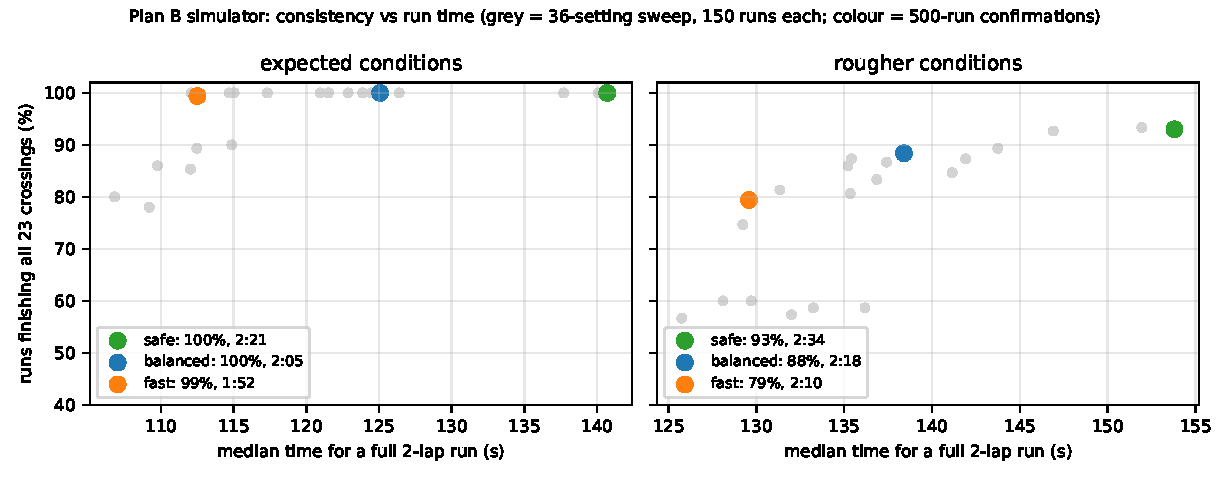
\includegraphics[width=\linewidth]{figs/planb_tradeoff.pdf}
\caption{Consistency against run time for every swept Plan B setting.}\label{fig:planbtrade}
\end{figure}

\begin{table}[H]\centering\footnotesize
\begin{tabular}{@{}lrr@{}}
\toprule
Assumption changed (setting ``balanced'', 300 runs each) & finish, expected & finish, rougher \\
\midrule
as designed & 100.0\,\% & 87.3\,\% \\
no barometer (vision height only) & 100.0\,\% & 82.7\,\% \\
detector range 8\,m & 100.0\,\% & 85.7\,\% \\
detector range 5\,m & 97.0\,\% & 47.0\,\% \\
no back-of-gate detection & 97.7\,\% & 64.3\,\% \\
gate fixes at 10\,Hz, +100\,ms latency & 99.7\,\% & 69.0\,\% \\
camera tilt unknown by 2\textdegree & 100.0\,\% & 83.0\,\% \\
camera tilt unknown by 5\textdegree & 92.3\,\% & 47.0\,\% \\
all of: no baro, 8\,m, no back view, 10\,Hz, 2\textdegree & 97.7\,\% & 45.0\,\% \\
\bottomrule
\end{tabular}
\caption{How much Plan B depends on its assumptions.}\label{tab:planbassump}
\end{table}

\begin{figure}[H]\centering
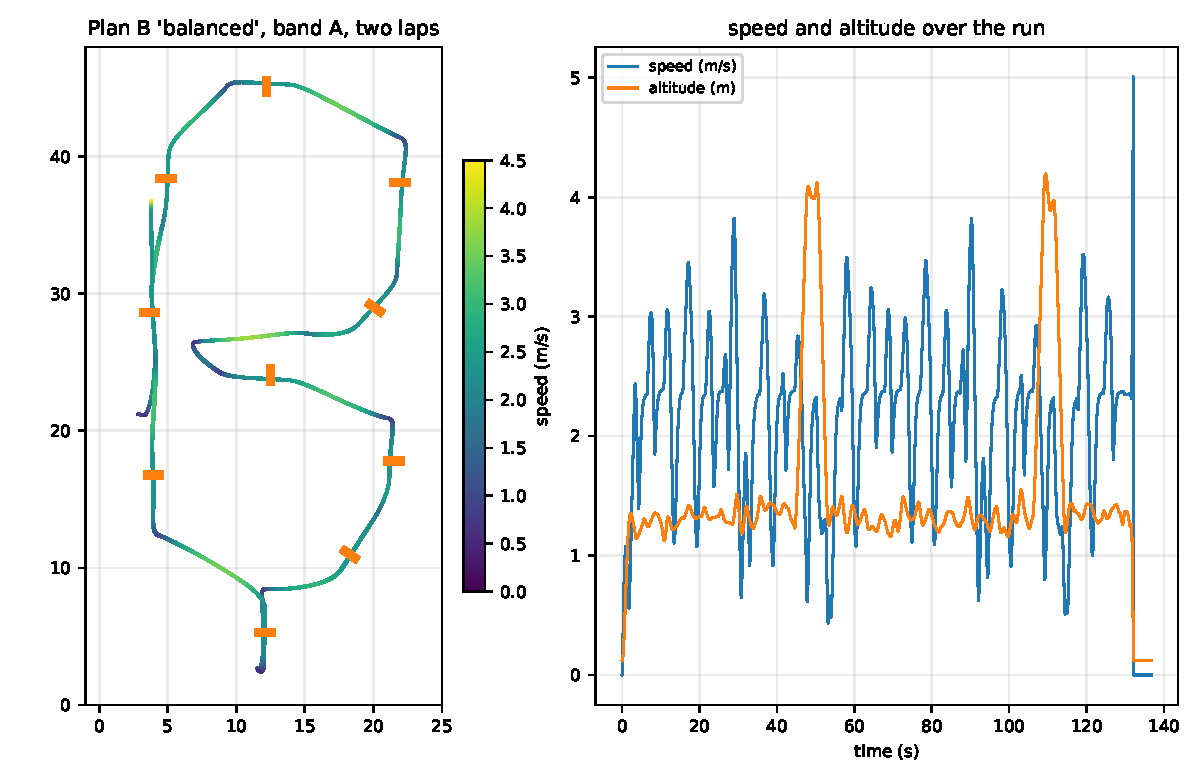
\includegraphics[width=0.95\linewidth]{figs/planb_path.pdf}
\caption{One simulated ``balanced'' run under expected conditions: split-S bypass around G6, climb to the upper opening of G9, two laps.}
\end{figure}

\begin{verdict}[Plan B verdict]
\begin{itemize}
\item \textbf{Recommended setting:} \textbf{``balanced''}. It finishes 100\,\% of runs under expected conditions and 88\,\% under rougher ones, in about \textbf{2:05} for two laps.
\item \textbf{If on-site conditions look rough:} use \textbf{``safe''} (2:21, 93\,\% under rougher conditions).
\item \textbf{Only after clean real runs:} try ``fast'' (1:52, 79\,\% under rougher conditions).
\item \textbf{Robustness under expected conditions:} it still finishes 98\,\% of runs with \emph{all} pessimistic assumptions at once.
\item \textbf{A barometer is optional.} Vision height relative to each gate teaches the thrust bias.
\item \textbf{The biggest single risk is camera tilt.} A \SI{5}{\degree} unknown tilt error drops finishing to 92\,\% (expected conditions) and 47\,\% (rougher). \textbf{Measure the tilt.}
\item \textbf{Under rough conditions,} a short detector range (5\,m), no back-of-gate detection and slow vision matter most.
\item \textbf{What limits run time:} the two forced turnarounds and the alignment pauses, not the cruise speed.
\end{itemize}
\end{verdict}

\begin{warnbox}[What this simulation does not cover]
\begin{itemize}
\item Real rotor aerodynamics near frames, and ground effect.
\item Detector false positives (orange pylons, red signage).
\item Wrong gate identity.
\item A real gate detector's accuracy. The test assumes a gate-relative pose with a few pixels of error.
\item Whether ANGLE mode is permitted; ask the organizers.
\item The airframe span; measure the real drone.
\end{itemize}
It shows that the Plan B \emph{logic and speed budget} are sound. It does not replace testing in the cage.
\end{warnbox}
}{}


%========================================================== GATE IDENTITY
\section{Knowing which gate is which}\label{sec:identity}

\subsection{The problem, and why it is not a perception problem}

The policy is told which gate it is flying at. In the simulator that arrives for
free. On the real course nothing publishes it, ten gates are identical
\SI{2.7}{m} squares, and \textbf{we asked the organizers whether we may mark them
and the answer was no}.

Measured on our own course: \textbf{34\,\% of frames have two or more gates in
view at once.} So ``look at the gate and recognise it'' is not available from
appearance, ever.

\begin{explain}[The reframe that makes this tractable]
Gate identity is not a perception problem. It is a \textbf{localisation}
problem. If you know where you are, identity is a lookup: project all ten gates
from the map and see which one you are pointed at. If you do not know where you
are, no amount of staring at an identical square will tell you.

Every published system reaches the same conclusion and none of them tries to
recognise gates individually.
\end{explain}

\subsection{What the policy actually reads}\label{sec:statevector}

Worth stating explicitly, because the argument below turns on it. Each frame is
51 numbers, and the policy reads \textbf{32 frames of history}, so 1632 inputs.

\begin{table}[H]\centering\footnotesize
\begin{tabularx}{\linewidth}{@{}p{1.6cm} p{3.1cm} X@{}}
\toprule
Index & Name & Meaning \\
\midrule
0--15 & \code{u0,v0 \dots u7,v7} & \textbf{Eight gate corners} as image positions, normalised by 640$\times$360. \textbf{$-1.0$ in both when not seen} \\
16--23 & \code{vis0 \dots vis7} & Is that corner seen? 1.0 or 0.0 \\
24--25 & \code{roll}, \code{pitch} & Attitude from the flight controller, radians \\
26--28 & \code{gx, gy, gz} & Gyro rates, body NED, clipped $\pm$8\,rad/s \\
29--31 & \code{vx, vy, vz} & Commanded body velocity, NED, clipped $\pm$20\,m/s \\
32--49 & \code{gate0 \dots gate17} & \textbf{Which gate is next} --- one slot set to 1.0 \\
50 & \code{lap\_frac} & Progress round the lap, $\mathrm{index}/17$ \\
\bottomrule
\end{tabularx}
\caption{The 51-number observation frame. Verified against the training code element by element (Section~\ref{sec:built}).}
\end{table}

The eight corners are \textbf{one gate only} --- the one being flown at, not all
ten. Corners 0--3 are the outer \SI{2.7}{m} frame, clockwise from top-left;
corners 4--7 are the inner \SI{1.5}{m} opening in the same order. Having both
rings is what encodes \emph{range}: their true sizes are known, so apparent size
gives distance.

Three things the policy is \textbf{not} given, which matter for what follows:
no distance, no position or altitude or heading (roll and pitch but not yaw),
and no sight of the \emph{next} gate. Everything beyond the gate in view comes
from the one-hot label and what the network memorised in training.

\begin{warnbox}[The consequence]
Nothing in indices 0--31 distinguishes gate~3 from gate~8. All ten are identical
squares. The \textbf{only} channel carrying course position is the one-hot in
32--49 --- which is 576 of the 1632 numbers once the 32 history frames are
counted, over a third of everything the network reads.
\end{warnbox}

\subsection{``The model will learn the order from simulation''}

A reasonable-sounding proposal was put forward: label the gates in simulation,
train on that, and the model will know the order on the real unlabelled gates.

The mechanical objection is that the label is an \textbf{input}, not an output.
Training with it does not teach the network the order; it teaches the network to
\emph{depend on being told} the order. At run time something must still supply
those 18 numbers, and a network cannot supply its own input.

But that is an argument, and arguments lose to measurements. So we measured it.

\paragraph{The experiment.} Gene's model, flown in \emph{his} simulator on
\emph{his} track --- his gate positions, his \SI{90}{\degree} camera, the
\SI{607.6}{g} drone --- the conditions where it works well. 512 drones at once,
\SI{20}{s} each. Identical physics, course, camera and seed across all five runs.
\textbf{The only thing changed is where the gate label comes from.}

\begin{table}[H]\centering\footnotesize
\begin{tabular}{@{}lrrrr@{}}
\toprule
Label source & \makecell{Gates per\\crash} & \makecell{Crashes /\\100 gates} & \makecell{Median\\lap} & \makecell{Laps\\completed} \\
\midrule
\textbf{Correct, as trained} & \textbf{26.9} & \textbf{3.4} & \textbf{7.45\,s} & \textbf{515} \\
Stuck on the start gate & 1.8 & 51.5 & --- & 0 \\
No label at all & 1.1 & 85.6 & --- & 0 \\
Random label each frame & 1.1 & 72.9 & --- & 0 \\
Off by one & 1.0 & 80.7 & --- & 0 \\
\bottomrule
\end{tabular}
\caption{The gate label is load-bearing. Raw data in \nolinkurl{~/aigp/eval/ctx/}; reproduce with \nolinkurl{run_ctx.sh}.}\label{tab:ctx}
\end{table}

\begin{verdict}[What this settles]
\begin{itemize}
\item \textbf{With the correct label the model is healthy}: \SI{7.45}{s} laps,
\SI{16}{m/s} at the gate, 515 complete laps, about 27 gates between crashes.
Exactly the performance it always had.
\item \textbf{Without a label it completes zero laps.} Not one, across any of the
four broken conditions. It crashes after roughly one gate.
\item ``Train with labels in simulation, then have nothing supplying them in
reality'' \emph{is} the ``no label at all'' row.
\item \textbf{Off-by-one is as bad as no label at all} (1.0 vs 1.1). This is not
only an argument for having a gate counter --- it is an argument for the counter
being \emph{right}. A counter that slips once is worth nothing.
\item \textbf{A frozen counter is the least-bad failure} (1.8). So when
confidence is lost, hold the last index rather than guess a new one. That is how
ours is built.
\end{itemize}
\end{verdict}

The instinct behind the proposal is not wrong, and is a real published
technique --- but it requires \emph{changing how we train}, not merely training
with labels present. Either drop the input entirely and force the network to
infer position from its 32 frames of history, or train a teacher with the
privileged label and distil it into a student that sees only what the drone
sees. Both work. Both have the same weakness: when the network's internal guess
is wrong there is no error signal, so it is confidently wrong. The approach
below at least knows when it is lost.

\subsection{What we build instead}

The published systems --- Swift\X, AlphaPilot\X\ and the 2026 dual pose-graph
work\X\ --- all share one shape: detect gate corners, solve a relative pose per
gate, match against the \emph{known map} in metric space, and fuse into a filter.
Swift states it plainly: each observation is assigned to ``the nearest gate in
the known trajectory layout''.

Two things we do differently, both because we measured rather than copied.

\paragraph{No visual-inertial odometry.} Every one of those systems leans on VIO.
We have one forward camera and a \SI{25}{W} budget. So we measured whether we
need it: a gate is in view \textbf{75--79\,\%} of frames, the worst gap is
\SI{1.5}{s} at \SI{5}{m/s}, and dead reckoning drifts \textbf{under a metre}
across that gap --- against gates that are \SI{7.54}{m} apart. VIO would be
solving a problem we do not have.

\paragraph{Throw away the PnP rotation.} Planar PnP is ill-conditioned near
head-on, which is where a racing drone spends its life. But we do not need its
rotation: the flight controller already gives us attitude, far more accurately.

\begin{table}[H]\centering\footnotesize
\begin{tabular}{@{}lrrr@{}}
\toprule
Corner noise & Range & Full 6-DOF PnP & \textbf{PnP translation + FC attitude} \\
\midrule
2\,px & 8\,m & 2.12\,m & \textbf{0.09\,m} \\
5\,px & 8\,m & 3.15\,m & \textbf{0.29\,m} \\
10\,px & 12\,m & 6.81\,m & \textbf{1.38\,m} \\
\bottomrule
\end{tabular}
\caption{Discarding the ill-conditioned half of the PnP solution is worth 23$\times$ at the operating point. This is not from the literature; it fell out of the accuracy test.}\label{tab:pnp}
\end{table}

\subsection{The pipeline}

\begin{enumerate}
\item \textbf{Detector} --- finds a gate's eight corners in the image.
\emph{Still to be built; needs real footage.}
\item \textbf{PnP} --- corners plus the known \SI{2.7}{m}/\SI{1.5}{m} geometry
give range and bearing to the gate. Planar PnP returns two mirrored solutions;
we pick by reprojection error and break ties with \textbf{gravity}, since gates
stand vertically and we know which way is down.
\item \textbf{Position} --- range and bearing, plus the flight controller's
attitude, plus the gate's known map position, give \emph{where we are}.
\item \textbf{Filter} --- carries position through the gaps by integrating thrust
and attitude, corrected by each fix. It also estimates \textbf{thrust scale},
which is what makes a barometer unnecessary --- and the barometer is unusable
anyway with the props spinning.
\item \textbf{Tracker} --- knowing where we are, project all ten gates and see
which one is ahead. Advance on a confirmed crossing. Fill the 18 one-hot slots.
\end{enumerate}

In one line: \emph{the gate looks this big and sits here in frame} $\rightarrow$
\emph{so it is \SI{8.3}{m} away, \SI{12}{\degree} left} $\rightarrow$ \emph{the
map says that gate is at (12.19, 45.11)} $\rightarrow$ \emph{so I am at
(10.4, 37.2)} $\rightarrow$ \emph{therefore this is gate 3} $\rightarrow$
\emph{set slot 35 to 1.0}.

\subsection{Evidence}\label{sec:built}

\begin{table}[H]\centering\footnotesize
\begin{tabularx}{\linewidth}{@{}p{4.3cm} X@{}}
\toprule
Check & Result \\
\midrule
Observation frame vs training code & \textbf{Exactly zero} difference, 51 numbers $\times$ 200 cases \\
History stack vs training code & \textbf{Exactly zero} difference across 1632 numbers \\
Projection vs training code & $3.9\times10^{-6}$\,px, zero visibility mismatches over 3200 corners \\
Policy in NumPy vs PyTorch & $2.5\times10^{-6}$ max error on the real checkpoint, \SI{126}{\micro s} per inference \\
Position, normal conditions & \textbf{0.88\,m median, 2.79\,m p95} against \SI{7.54}{m} gate separation \\
\dots with 20\,\% thrust error & 0.88\,m / 2.79\,m (thrust scale learned 0.895 vs true 0.900) \\
\dots drag model 2$\times$ wrong & 0.80\,m / 3.01\,m \\
\dots 10\,px corner noise & 1.01\,m / 2.38\,m \\
\dots \SI{7}{m} detector range & 0.77\,m / 2.29\,m \\
\dots \SI{12}{m/s} flight & 0.77\,m / 1.57\,m \\
Dead reckoning with no fixes & 88.9\,m / 177\,m --- useless alone, which is the point \\
Gate counting, 17 conditions & 22/22 crossings, zero errors (50\,\% dropout, 20 false positives/s, \SI{100}{ms} latency, 1\,m pose noise) \\
\bottomrule
\end{tabularx}
\caption{Everything above is reproducible with \code{python run\_all.py} in \nolinkurl{flight/}.}
\end{table}

\begin{warnbox}[The one known limit: heading drift]
The position fix is computed \emph{using} our heading, so a wrong heading
corrupts the fix directly and no filter can recover --- the measurement itself is
wrong. Measured tolerance:

\begin{center}\footnotesize
\begin{tabular}{@{}lrrl@{}}
\toprule
Yaw drift & Median & p95 & \\
\midrule
\SI{0.05}{\degree\per\second} & 0.28\,m & 0.97\,m & fine \\
\SI{0.5}{\degree\per\second} & 0.90\,m & 2.81\,m & fine \\
\SI{1.0}{\degree\per\second} & 1.47\,m & 6.81\,m & \textbf{breaks} \\
\bottomrule
\end{tabular}
\end{center}

So it tolerates about \SI{0.5}{\degree\per\second} and fails near
\SI{1}{\degree\per\second}. A calibrated Betaflight gyro should be an order of
magnitude better than that, but this is now a specific number to \textbf{verify
from the measurement flight} rather than assume.
\end{warnbox}


%------------------------------------------------------------------------
%========================================================== TECHNICAL GAPS
\section{Technical gap register}\label{sec:gaps}

\subsection{First, what Betaflight actually is}

Several gaps below are ``Betaflight things'', so here is the minimum needed to read them.

\begin{explain}[The flight controller, in plain terms]
The \textbf{flight controller} is a small circuit board on the drone with a gyroscope on it, running
firmware called \textbf{Betaflight}. Its job is narrow and fast: take four numbers --- throttle,
roll, pitch, yaw --- several thousand times a second, and spin the four motors so the drone does what
those numbers ask. It handles the violent, millisecond-scale balancing that keeps a quadcopter in
the air. We do not have to write that, and we could not do it better.

Normally those four numbers come from a \textbf{radio receiver} wired to the flight controller,
listening to a human pilot's remote control.

\textbf{MSP} (MultiWii Serial Protocol) is simply a message format for talking to the flight
controller down a serial wire. Betaflight speaks it. The feature we need is called \textbf{MSP
override}: while a switch on the pilot's remote is flipped on, Betaflight takes its four stick
numbers from MSP messages --- from our Jetson --- instead of from the radio. Flip the switch off and
the pilot has the drone back, immediately, in firmware. That is our kill path.

Two more terms that appear below:
\begin{itemize}
\item \textbf{ACRO and ANGLE} are flight modes. In \textbf{ACRO}, stick position means \emph{rate of
rotation}: hold the stick over and the drone keeps rolling; centre it and it stops rolling but stays
tilted wherever it ended up. In \textbf{ANGLE}, stick position means \emph{lean angle}: centre the
stick and it returns to level by itself. Our trained policy outputs rotation rates, so it needs
ACRO. Plan~B wants ANGLE, because ``hold still and hover'' is then almost free.
\item \textbf{Blackbox} is Betaflight's built-in flight recorder. It logs throttle, gyro, motor
outputs and battery voltage during a flight, and you download it over USB afterwards. Almost every
measurement we need about the drone comes out of it.
\end{itemize}
\end{explain}

\subsection{Gap register}

Effort is one person's working time. ``Blocks'' names what cannot start until this is done.

{\setlength{\tabcolsep}{3pt}\begin{longtable}{@{}p{0.85cm} p{3.9cm} p{6.5cm} p{1.45cm} p{1.95cm}@{}}
\toprule
ID & Gap & What it means, and why it matters & Effort & Blocks \\
\midrule\endhead
\multicolumn{5}{@{}l}{\textbf{A --- Flight controller and the link to it} \emph{(much reduced: the organizers ship the protocol layer)}}\\
\midrule
A0 & Copy \code{~/target/} off a board & \code{scp -r dcl@192.168.55.1:~/target ./}. Until somebody does this, nobody else can develop against the fake flight controller. & 10 min & All adapter work \\
A1 & Adapter, not protocol & MSP framing is provided. We write the layer that turns policy output into \code{RCTransmitter.set\_control()} calls. & 4\,h & Everything autonomous \\
A2 & Free the serial port & \code{sudo setup\_jetson\_uart.sh -{}-apply}, once per board. Linux runs a login console on that port by default. \textbf{Skipping this looks exactly like a dead flight controller.} & 5 min & Any link at all \\
A3 & Rate curve inversion & \textbf{Still ours.} Betaflight maps stick to rotation rate along a curve (\code{rc\_rate}, \code{super\_rate}, \code{expo}), gentle in the middle and aggressive at the ends. Our policy speaks radians per second. A linear approximation is wrong by tens of percent mid-range. & 4\,h & Accurate control \\
A4 & Throttle curve inversion & \textbf{Still ours.} Same for throttle (\code{thr\_mid}, \code{thr\_expo}). & 1\,h & Height control \\
A5 & Sign and axis mapping & \textbf{Still ours, and the most dangerous item here.} Isaac is forward-left-up, Betaflight is forward-right-down, plus channel order. A reversed sign flips the drone on takeoff. Verify one axis at a time, props off. & 2\,h & Any flight \\
A6 & Watchdog: configure and verify & \code{RCTransmitter} already has one, in its own thread. Set the timeout, then prove it against \code{fake\_fc.py}'s frozen mode. & 1\,h & Safety sign-off \\
A7 & \textbf{Loop rate mismatch} & Organizers: attitude at 30--50\,Hz is realistic, a hard real-time loop is not. Our policy runs at 60\,Hz and eats gyro as input. Measure, then match the simulator to it. & 2\,h & \textbf{Training validity} \\
A8 & Gyro units unverified & Sources conflict: raw counts at 16.4 per \si{\degree\per\second} versus already in \si{\degree\per\second}. \textbf{Verify empirically} --- the wrong choice is a silent 16$\times$ error. & 30 min & Sensor fusion \\
A9 & Arming flow & \code{msp\_bench.py demo} clears an MSP arming lock, arms, then re-asserts it; Betaflight also blocks arming while an MSP client is connected. Read their code and copy the sequence. & 2\,h & Any real run \\
A10 & Override mask: verify, do not assume & The mask\,=\,11 finding (throttle not overridden) came from \emph{another team's} dump. Since \code{demo} drives throttle successfully, ours may already be right. Check \code{diff all} on our drone. & 10 min & Autonomous hover \\
A11 & ANGLE mode not assigned & Flies ACRO; Plan~B needs ANGLE. CLI-assignable --- confirm it is permitted. & 15 min & Plan~B \\
A12 & Blackbox not configured & Must be on and recording gyro debug data, or the measurement flight yields nothing. & 15 min & All diagnostics \\
A13 & Camera/IMU time sync & \textbf{No hardware sync line exists on this carrier.} Must be solved in software, and the exposure must be pinned first or auto-exposure moves the capture instant every frame. & 4\,h & Latency measurement \\
\midrule
\multicolumn{5}{@{}l}{\textbf{B --- Onboard software}}\\
\midrule
B1 & Capture with \emph{real} timestamps & Viewers exist. But \code{cv2.VideoCapture} discards the hardware capture timestamp and gives arrival time with tens of ms of jitter. Use the GStreamer path where timing matters. & 4\,h & Perception \\
B1b & \textbf{Image processor needs a display} & Colour, auto-exposure and white balance run in NVIDIA's ISP, which needs a graphics context a plain SSH session lacks. Headless gives flat, un-exposed frames \emph{by design}. Arrange a display context, or design for minimally-processed frames. & 4\,h & Usable images \\
B2 & \textbf{No framework on the board} & Confirmed: OpenCV, NumPy, pyserial, python3-gi --- no PyTorch. The NumPy policy runtime is now \emph{mandatory}. The detector must go to ONNX via OpenCV's DNN module or TensorRT. Never \code{pip install opencv-python}: it silently breaks the camera pipeline. & 3\,h & Plan~A \\
B3 & No gate counter & The ``which gate is next'' input has no source on the real drone. & 1 day & Plan~A \\
B4 & No takeoff routine & The policy was trained starting \emph{in the air} near a gate. The real race starts on the floor. Something must take off, stabilise, and hand over. & 4\,h & Any real run \\
B5 & Crash and abort logic is simulator-era & The existing logic auto-re-arms after a crash, which is a simulator behaviour and dangerous on a real drone. & 3\,h & Safety sign-off \\
B6 & No onboard logging standard & Every flight needs a synchronised record of inputs, outputs and detections, or we cannot diagnose anything. & 2\,h & All learning \\
B7 & Compute budget unverified & Detector plus policy plus capture, at 25\,W, at the target frame rate. Unknown until measured. & 2\,h & Loop rate \\
\midrule
\multicolumn{5}{@{}l}{\textbf{C --- Perception}}\\
\midrule
C1 & Detector has never seen a real gate & Existing detectors were tuned on simulator images. See Section~\ref{sec:detect}. & 2 days & Any autonomy \\
C2 & Camera not calibrated & The spec states no calibration will be provided, and it is a screw-mount lens. & 1\,h & Perception accuracy \\
C3 & Camera tilt unknown & It is adjustable, even in flight, so it is a choice we must make and then measure. A \SI{5}{\degree} error took crashes to 32 per 100 gates. & 30 min & Perception accuracy \\
C4 & \textbf{Sensor mode may not exist} & The carrier wires only \textbf{two of the camera's four data lanes}, capping resolution $\times$ framerate. \code{v4l2-ctl -{}-list-formats-ext} is the truth, not the datasheet. The \SI{75}{\degree} figure is quoted for 1920$\times$1080 at 60\,fps --- if that mode is missing, our field of view is wrong before we start. & 10 min & Everything perception \\
\midrule
\multicolumn{5}{@{}l}{\textbf{D --- Simulator fidelity}}\\
\midrule
D1 & Thrust-to-weight is a guess & Hover throttle assumed 25.5\,\%. Worth 58 crashes per 100 gates if wrong by 10\,\%. & 5 min & Training validity \\
D2 & Inertia and rate response wrong & 5-inch airframe values on an 8-inch drone; see the warning in the status section. & 4\,h & Training validity \\
D3 & Zero latency modelled & The most damaging single factor found: \SI{50}{ms} alone took crashes from 2 to 55 per 100 gates. & 3\,h & Training validity \\
D4 & No drag model & Significant above \SI{10}{m/s}. & 3\,h & Training validity \\
D5 & Perfect vision assumed & The simulator hands the policy exact gate corners with no noise, no dropouts and never the wrong gate. This is the largest single difference between simulation and reality. & 1 day & Transfer \\
D6 & Course map: official table in hand & The official coordinates confirm $85\times165$\,ft and our corrected track matches exactly. \textbf{Still survey the as-built placement} --- a 7.5\,\% scale error alone took crashes from 2 to 15.5 per 100 gates. & 2\,h & Training validity \\
D7 & \textbf{Policy rate may be too fast} & Simulator runs a 60\,Hz policy; real gyro feedback may be 30--50\,Hz. Set decimation to the measured rate \emph{before} the long training run. & 1\,h & Training validity \\
\midrule
\multicolumn{5}{@{}l}{\textbf{E --- Operations}}\\
\midrule
E1 & No compiler on the laptop & \textbf{Downgraded.} The Betaflight software-in-the-loop build is no longer needed --- the organizers' \code{fake\_fc.py} is pure Python and does the job better. & 10 min & nothing now \\
E2 & Practice slots unknown & Flight time is rationed and scheduled. Everything must be planned around the slot list. & --- & All planning \\
E3 & Battery and propeller count unknown & The real limit on how many attempts we get. & --- & Risk budget \\
\bottomrule
\caption{Technical gap register as of 17 September, after reading the organizers' Orin NX guides. Nothing here is a criticism of the existing code --- almost all of it was written for the virtual qualifier, which was a different race with a different interface. The A-series shrank considerably once it became clear the organizers ship the protocol layer themselves.}\label{tab:gaps}
\end{longtable}}

%========================================================== WORKSTREAMS
\section{The plan, organised as parallel workstreams}\label{sec:ws}

The mistake to avoid is queueing everything behind the flight-controller link. Only one workstream
actually depends on it. Three others need no software at all and should start the same hour.

\begin{table}[H]\centering\footnotesize
\begin{tabularx}{\linewidth}{@{}p{1.1cm} p{3.0cm} X p{2.4cm}@{}}
\toprule
Stream & Name & Content & Waits for \\
\midrule
\textbf{WS-1} & Link and control & MSP implementation, curve inversion, watchdog, bench validation (gaps A1--A12) & \textbf{Nothing.} This is the critical path \\
\textbf{WS-2} & Vehicle characterisation & Weigh, balance, measure; the piloted measurement flight; hover thrust, rate response, drag, battery sag (D1--D4) & \textbf{Nothing} --- a human pilot and a blackbox log need no code \\
\textbf{WS-3} & Perception & Camera bring-up, calibration, data capture, labelling, detector, gate counter (B1, B3, C1--C4, D5) & Camera only \\
\textbf{WS-4} & Course survey & Tape-measure every gate from a fixed datum; reconcile with both documents; build the map (D6) & \textbf{Nothing} --- hall access and a tape measure \\
\textbf{WS-5} & Simulator and training & Fold measurements in; cloud training with randomised unknowns; evaluate with the stress harness & \textbf{Nothing} --- starts with wide randomisation \\
\textbf{WS-6} & Integration and flight test & The bring-up ladder, in practice slots & WS-1, plus WS-3 and WS-4 for gate work \\
\textbf{WS-7} & Plan~B & The slow stop-and-line-up controller & WS-1, WS-3 \\
\textbf{WS-0} & Operations & Slots, batteries, organizer questions, installs, logistics & \textbf{Nothing} \\
\bottomrule
\end{tabularx}
\caption{Eight workstreams. Five of the eight can start immediately and in parallel.}
\end{table}

\begin{takeaway}[How to staff this]
Put your strongest systems person on \textbf{WS-1} alone, with a second person reviewing the sign
and axis conventions --- a reversed sign there flips the drone on takeoff, and it is the single most
common first-flight failure in this whole field.

\textbf{WS-2} needs the pilot plus one engineer, and it is the cheapest high-value work available:
one battery, one log, and the simulator stops guessing.

\textbf{WS-4} is two people and ninety minutes, and it retires a risk worth 15 crashes per 100
gates. Do it on day one and do it again before the scored days.

\textbf{WS-3} is the longest pole after WS-1 and it is mostly patient work --- capture, label, train,
measure. Start the capture the hour the camera produces a frame.
\end{takeaway}

%========================================================== PROCEDURES
\section{Field procedures}\label{sec:proc}

\subsection{P1 --- Camera calibration}
\begin{enumerate}
\item Confirm the sensor mode first (gap C4). The \SI{75}{\degree} figure applies to 1920$\times$1080
at 60\,fps. If our pipeline captures another mode, the field of view is different before we start.
\item Print a checkerboard or ChArUco target and \textbf{glue it to something rigid and flat}. A
curled printout produces a confident, wrong calibration.
\item Capture 30--50 views at the race exposure and gain settings: target near and far, tilted in
both axes, in all four corners of the frame.
\item Solve for focal length, principal point and distortion (OpenCV). Expect a reprojection error
below about half a pixel; if it is worse, the target moved or the board is not flat.
\item \textbf{Sanity check independently:} tape measure flat against a wall, camera exactly
\SI{2.00}{m} away, and confirm the width spanned matches the focal length you solved for.
\item Record the result with the date and the specific drone. The four airframes may not match.
\end{enumerate}

\subsection{P2 --- Camera tilt}
\begin{enumerate}
\item Set the drone on a surface you have confirmed is level with a spirit level.
\item Measure the camera mount angle with a phone inclinometer held against the lens face or the
bracket. Repeat three times and take the median; this is easy to get wrong by a couple of degrees.
\item Cross-check optically: place a target at a known height at a known distance and confirm it
lands where the calibrated model predicts.
\item Tilt is adjustable, so \textbf{decide} it: a lower tilt (around \SI{10}{\degree}) suits Plan~B's
slow, near-level flight; a higher tilt (around \SI{20}{\degree}) suits fast forward-leaning flight.
Choose, set, measure, and write it down. Then use that number in the simulator.
\end{enumerate}

\subsection{P3 --- Vehicle diagnostics: one battery, one log}\label{sec:diag}

This is the highest-value thirty minutes of the week. Fly it with a human pilot, with blackbox
logging switched on, in this order. It needs no autonomy software at all.

\begin{table}[H]\centering\footnotesize
\begin{tabularx}{\linewidth}{@{}p{0.6cm} p{4.4cm} X@{}}
\toprule
\# & Manoeuvre & What it yields \\
\midrule
1 & Armed on the ground, 10\,s idle & Gyro noise floor; vibration spectrum; motor idle value \\
2 & Stable hover at \SI{1.5}{m} for 20\,s & \textbf{Hover throttle} --- gap D1, the most valuable number available. Also a ground-effect reference \\
3 & Three sharp rolls, three pitches, three yaws, settling between each & \textbf{Rate response}: rise time, overshoot, peak angular acceleration, per axis --- gap D2. This is what replaces guessing the inertia \\
4 & Full-throttle vertical climb, 1.5\,s, then recover & \textbf{Maximum thrust} and true thrust-to-weight \\
5 & Hold about \SI{20}{\degree} of pitch down a straight until the speed stops rising & \textbf{Drag} --- gap D4. Drag coefficient $\approx m g \tan\theta / v^2$ \\
6 & Hover again for 20\,s near the end of the pack & \textbf{Battery sag}: how much hover throttle rises as the pack empties \\
7 & Land, disarm, download the log, and save a \code{diff all} from the CLI & The settings dump. Do not skip this; it is the thing that will be missing at 2\,a.m.\ \\
\bottomrule
\end{tabularx}
\end{table}

Repeat manoeuvre~2 on every airframe you might fly. Hover throttle is the number the whole simulator
hangs from, and four supposedly identical drones are rarely identical.

\subsection{P4 --- Latency}
Latency is the most damaging single factor in the durability study, and it is also the one people
estimate instead of measuring. Measure it.
\begin{enumerate}
\item Synchronise the clocks first (gap A12), or the answer is meaningless.
\item Put a bright LED in the camera's view, wired so the Jetson can switch it.
\item Flash it, and record: the time the Jetson commanded the flash; the timestamp of the first frame
showing it lit; the time the detector produced an output; the time the command went out over MSP; and
the time the gyro first responded.
\item That chain gives you each stage separately, which matters --- knowing the total is \SI{90}{ms}
is useful, knowing that \SI{60}{ms} of it is the detector tells you what to fix.
\item Feed the measured total, and its variation, into the simulator as a randomised band.
\end{enumerate}

\subsection{P5 --- Course survey}
\begin{enumerate}
\item Choose a datum: a permanent corner as the origin, plus a second fixed feature to define the
direction of the $x$ axis. Mark both with tape and photograph them.
\item For each gate, measure the \textbf{base of both uprights} from the datum. Two points give you
the centre \emph{and} the heading in one operation, which is far more reliable than measuring an
angle directly.
\item Record the bottom-bar height for one gate of each type, and confirm the double gate's upper
opening centre.
\item Note what the drawing does not show: pylons, netting, lighting rigs, anything above \SI{4}{m}.
\item Convert to the simulator's frame and difference against \emph{both} the organizer table and the
drawing. Reconcile every gate that differs by more than \SI{0.25}{m} before training on it.
\item Re-measure every morning and before every scored run. Ask what tolerance gates are re-placed
to; that number becomes the gate-jitter range in training.
\end{enumerate}

\subsection{P6 --- Gate detection and data labelling}\label{sec:detect}

This deserves its own treatment, because it is the largest difference between our simulator and
reality, and it is the workstream most likely to be underestimated.

\begin{explain}[Why this is hard, when the simulator makes it look easy]
In the simulator, the policy is handed the eight corners of the gate as exact pixel coordinates,
computed by projecting the gate's known geometry through a perfect pinhole camera. There is no noise.
Corners are never missed. It is never the wrong gate. Visibility is known exactly.

On the real drone, every one of those is false. You have a compressed image of an orange-and-white
frame against a cluttered hall, with motion blur, a rolling shutter that skews fast-moving objects,
changing light, other gates in frame, orange pylons that look like gate material, and a detector that
will sometimes return nothing and occasionally return something confidently wrong.

\textbf{Closing this gap has two halves, and the second is the one teams skip:} make the detector as
good as is reasonable, \emph{and} make the policy tolerant of a realistic detector by reproducing the
detector's \emph{measured} error statistics inside the simulator. Perfect detection is not
achievable; a policy that degrades gracefully when detection is imperfect is.
\end{explain}

\paragraph{Stage 0 --- classical detector, first hour.}
Tune the existing colour-and-geometry detector on real frames --- it lives in \code{vision/} as
\code{snake\_gate\_detector}, and \code{tools/hsv\_tuner} adjusts its colour thresholds. No data, no
training, no installation. It will be noisier
and shorter-ranged than a learned detector, but it is available immediately and it is the fallback
that cannot fail to be ready. Plan~B tolerates a noisy detector far better than Plan~A does.

\paragraph{Stage 1 --- capture, starting the hour the camera works.}
Data capture is the bottleneck, so begin it before you need it. Capture must cover:
\begin{itemize}
\item distances from about \SI{1}{m} to \SI{15}{m}, and all approach angles including oblique;
\item \emph{every} gate on the course --- the backgrounds differ, and that is what a detector learns;
\item gates partially cut off by the frame edge, and two gates overlapping;
\item the double gate, from below and from the upper approach;
\item backlit and shadowed conditions, and whatever the lighting does across a day;
\item \textbf{negatives}: frames with no gate, and frames containing confusers --- orange pylons, red
signage, other drones, people;
\item \textbf{motion blur}, which means recording every manual pilot flight. Hand-carried footage is
easy to collect but is missing exactly the degradation that matters in flight.
\end{itemize}

\paragraph{Stage 2 --- labelling, done cheaply.}
Labelling is where teams lose a day. Three techniques cut the work by roughly five to ten times:
\begin{enumerate}
\item \textbf{Auto-label, then correct.} Run the classical detector over all footage and keep its
output as draft labels. Correcting a drawn box is far faster than drawing one.
\item \textbf{Geometric auto-labelling --- the big win.} We know the gate's exact geometry
(\SI{2700}{mm} outer, \SI{1500}{mm} inner) and, after the survey, exactly where each gate is. If the
camera pose for a frame is known, the eight corners project into the image exactly --- the label is
free and pixel-perfect. Bootstrap it: hand-label around 40 frames, solve the camera pose from those
by PnP, then track along the video and re-project labels for every frame in between. This is how an
afternoon produces thousands of labelled frames instead of a few hundred.
\item \textbf{Label what the policy actually needs.} The observation wants eight keypoints plus
visibility flags --- not bounding boxes. Keypoint labelling is slow. A hybrid is cheaper: let a
learned model find the gate as a box, then fit the quadrilateral inside it with classical line
fitting. Much less labelling, and \code{vision/yolo\_hybrid\_gate\_detector.py} is already shaped
this way.
\end{enumerate}
For a single, visually distinctive object class, fine-tuning a pretrained detector typically needs
\textbf{300--800 well-chosen labelled frames}, not tens of thousands. Spend the effort on coverage
and on the hard cases, not on volume.

\paragraph{Stage 3 --- train and deploy.}
Fine-tune on the laptop GPU; it is a small model and takes minutes. Then build the accelerated engine
\textbf{on the Jetson itself} --- these are specific to the device and software version and cannot be
prepared in advance. Budget real time for this at the venue.

\paragraph{Stage 4 --- measure the detector, because this is what feeds the simulator.}
The useful metrics are not the ones detector papers report. Measure:
\begin{itemize}
\item detection rate against distance --- what \emph{is} our reliable range?
\item corner pixel error against distance and viewing angle, as a median and a 95th percentile;
\item false positives per frame, and specifically what triggers them;
\item how often the identity is wrong;
\item throughput and latency at \SI{25}{W}.
\end{itemize}
Get ground truth by placing the drone at tape-measured positions relative to a gate: those frames have
exactly known corner positions, so the error can be measured rather than estimated.
\code{tools/eval\_detectors.py}, \code{tools/eval\_gate\_pose.py} and \code{tools/vision\_rate.py}
exist for this.

\paragraph{Stage 5 --- close the loop.}
Feed those measurements back as the simulator's vision model: pixel noise as a function of distance,
dropout rate, maximum range, frame rate, latency. Then retrain. This is the step that converts a
detector measurement into a policy that survives a real detector, and it is the reason Stage~4 is not
optional.

\paragraph{The gate counter.}
Separately from detection: maintain the expected gate number, predict where that gate should appear
using the surveyed map, and accept a detection only if it lands near the prediction. Advance the
count on a confirmed pass, with a short lockout so one crossing cannot count twice. \textbf{Encode
explicitly that the double gate counts twice per lap} --- one physical gate carrying two different
numbers is where a counter desynchronises. If the expected gate is not seen for a while, widen the
search, then fall back to a hold; never silently re-label, and log every re-association. Test all of
this offline by replaying a hand-carried lap before it ever flies.

%========================================================== SCHEDULE
\section{Schedule and decision gates}\label{sec:schedule}

\begin{table}[H]\centering\footnotesize
\begin{tabularx}{\linewidth}{@{}p{1.5cm} p{3.2cm} X@{}}
\toprule
Day & Goal & Exit criterion \\
\midrule
Thu 17 & We can command the drone, and we know the course & Bench test with propellers off passes on all four axes; piloted measurement flight logged; hover throttle known; course surveyed; overnight training launched \\
Fri 18 & We can see and count gates & Detector working on real gates; gate counter verified offline against recorded footage; autonomous hover; station-keeping in front of one gate \\
Sat 19 & \textbf{A complete lap, by any means} & One clean Plan~B lap. This puts a floor under the score. Plan~A begins with the speed limiter at minimum \\
Sun 20 & Rehearsal and freeze & Both plans rehearsed under run conditions; gates re-measured; configuration frozen; \textbf{Plan~A go/no-go} \\
Mon 21 & \textbf{Scored} & First slot: most reliable configuration, flown slowly, to bank gates. Then step up \\
Tue 22 & \textbf{Scored} & Improve on the banked score. Never risk the drone before a valid run exists \\
\bottomrule
\end{tabularx}
\end{table}

\textbf{Plan~A go/no-go, Sunday.} All three must hold:
\begin{enumerate}
\item it has flown at least three gates autonomously on the real drone, more than once;
\item its observations have been checked against the real camera and the real flight-controller
curves;
\item its failure mode is a safe hold, not a flyaway.
\end{enumerate}

\begin{warnbox}[The scoring rule that should drive every decision]
Ranking is by \textbf{maximum number of gates passed}; time is only the tie-break; and it is the best
run across the final two days. A slow run that completes therefore beats a fast run that ends at gate
four. Bank a score first. Push afterwards. Do not let the last day be the first time we have completed
a run.
\end{warnbox}

%========================================================== QUESTIONS
\section{Questions still open for the organizers}

The specification answered several questions that Revision~1 listed. Answered: the interface is MSP
over UART, with demo software provided; Betaflight CLI access covers rates, PIDs and filters but not
reflashing; camera tilt is adjustable in flight; exposure and gain are controllable; no calibration
matrices are provided; a valid run is two laps with no human pilot intervention; manual override
always supersedes autonomy; practice is in scheduled slots.

Still open:
\begin{enumerate}
\item May we assign an ANGLE mode switch, and change \code{msp\_override\_channels\_mask}, the rate
curve and the throttle curve?
\item May we place tape or markers on the gates to identify them? \textbf{A yes largely removes the
gate-counting problem}, so ask early.
\item Who arms the drone for a scored run? Does arming and enabling override before the start line
count as intervention?
\item Is there a maximum run duration? How many scored attempts per team per day?
\item Are gates re-placed between runs, and to what tolerance?
\item Are gates counted only in order --- does skipping one stop the count? Is a run that crashes
after $N$ gates scored as $N$?
\item Which camera sensor mode is the \SI{75}{\degree} figure quoted for, and can we change modes?
\item Are all four drones on identical firmware and configuration? Is a barometer fitted?
\item Where do we get the camera and serial demo applications?
\item Exact as-built gate heights, and the upper opening height of the double gate.
\end{enumerate}


%------------------------------------------------------------------------
\appendix
\section{Laptop environment (installed 16 Sep)}
\begin{itemize}
\item \textbf{Hardware:} RTX 4060 Laptop (8\,GB), 15\,GB RAM (WSL sees 7.6\,GB), 16 cores, WSL Ubuntu 26.04, no passwordless sudo.
\item \textbf{Missing:} no compiler at all --- \code{gcc}, \code{g++}, \code{make}, \code{cmake} and \code{ffmpeg} are absent, which blocks building the Betaflight software-in-the-loop simulator. \code{venv-client} has no \code{pip}. One command fixes both: \code{sudo apt install -y build-essential cmake ffmpeg poppler-utils}, then \code{python -m ensurepip}.
\item \textbf{Repo:} \code{~/Downloads/ai-grand-prix/AI_GP}, branch \code{isaacsim}, read-only for us.
\item \textbf{Flight client:} \code{~/aigp/venv-client} (Python 3.12, CUDA torch, ultralytics, OpenCV, pymavlink, pytest, tensorboard). The client test suite: 441 pass, 79 fail, 1 skip; the failures are in retired VQ code or are minor drift.
\item \textbf{Isaac:} \code{source ~/aigp/isaac_env.sh}. Isaac Sim 4.5, Isaac Lab 2.1 (\code{~/aigp/IsaacLab}), skrl 1.4.2, torch 2.5.1+cu121.
\begin{itemize}
\item Pins: numpy$<$2, transformers$<$4.50, warp-lang$<$1.8, gymnasium$<$1.2.
\item System libraries were unpacked from \code{.deb} files into \code{~/aigp/syslibs}.
\end{itemize}
\item \textbf{Scratch copies:}
\begin{itemize}
\item \code{~/aigp/idr_smoke}: original code.
\item \code{~/aigp/idr_A}, \code{idr_B}: bug A/B test.
\item \code{~/aigp/idr_exp}: bug fix, used for all experiments.
\end{itemize}
\item \textbf{Tools and results:} \code{~/aigp/tools/eval_policy.py}, \code{stress_eval.py}, \code{make_figs.py}; results in \code{~/aigp/eval/}.
\end{itemize}

\section{Sources}
\begin{itemize}
\item VADR-TS-005 PQ Technical Specification, issue 00.02 (2026-09-03); AI Grand Prix welcome packet.
\item theaigrandprix.com (home/FAQ, previous updates, official rules); public PQ spec TS-004; VQ2 spec TS-003.
\item Organizer gate-coordinate table ``Drone\_Race\_Track\_Gate\_Coordinates\_with\_doublegate\_5800.pdf'', as published in another team's repository.
\item \code{github.com/JCorbin406/AIGP-Physical-Qualifier} (``AI of Sauron''): FC dump, MSP notes, camera calibration, on-site confirmations. No license, so facts are used and no code.
\item Betaflight 4.4.3 source, \code{src/main/rx/msp_override.c}, \code{src/main/rx/msp.c}.
\item kousheekc/isaac\_drone\_racer (BSD-3); Isaac Lab 2.1; skrl 1.4.2.
\item Kaufmann et al., ``Champion-level drone racing using deep reinforcement learning'', \emph{Nature} 2023; Xing et al., CoRL 2024 (imitation plus RL for vision-based racing).
\end{itemize}

\end{document}
